\documentclass[../main.tex]{subfiles}
\graphicspath{{resources/}{resources/pcb_res}}

\begin{document}

\section{Eszköz (elektronikai és beágyazott szoftverének) tervezése és összeállítása}
    \subsection{Elektronikai tervezés}
        Az elektronikai tervezést 3 fázisra és az utolsó fázis hibáinak kijavítására bontottam le. Az első fázis első lépései között szerepelt az Ebay-ről vásárolt eszközök tesztelése: működik-e mindegyik, programozható-e a fejlesztői lap, konfigurálható-e a Wifi modul, stb.
        
        Második lépésként a mikrovezérlő lábkiosztása (\ref{fig:stm32f103_pinout}. ábra) alapján kiválasztottam a lábak általam használt funkcióit. 
        
        % https://os.mbed.com/users/hudakz/code/STM32F103C8T6_Hello/wiki/Homepage
        \begin{figure}[h!]
            \centering
                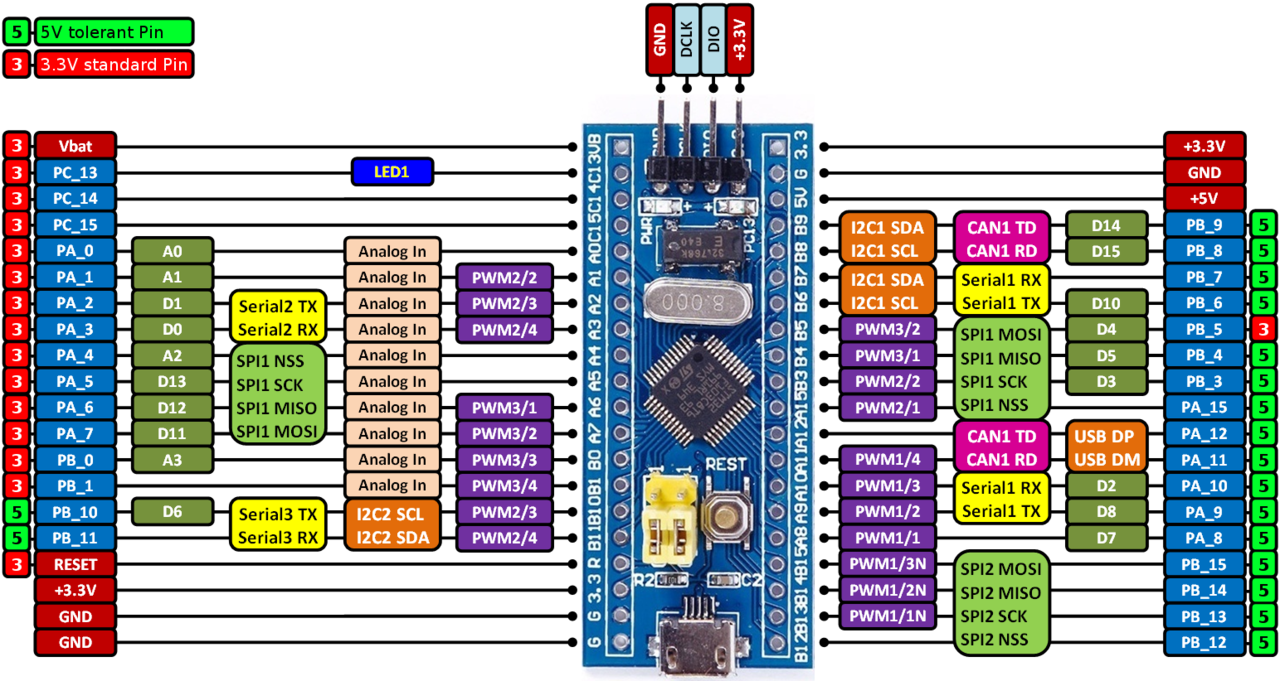
\includegraphics[width=14cm]{resources/pcb_res/stm32f103c8t6_pinout.png}
            \caption{STM32F103C8T6 fejlesztői lap pinout-ja}
            \label{fig:stm32f103_pinout}
        \end{figure}
        
        A PB\_0-s lábat választottam a LED sor vezérlő lábnak, és a PA\_9, PA\_10 (TX,RX) lábakat pedig Wifi modullal kommunikáló UART lábaknak. Minden modulra az előírt tápfeszültséget kötöttem, illetve az összes földpotenciált összehuzaloztam, ezzel egy közös földpontot létrehozva. A ESP-01-s modul pinoutja (\ref{fig:eps01_pinout}. ábra) alapján az UART lábakat is összekötöttem a megfelelő módon: a mikrovezérlő RX lábát (PA\_10) a Wifi modul U0TXD lábával és mikrovezérlő TX lábát (PA\_9) a Wifi modul U0RXD lábával. 
        
        \begin{figure}[h!]
            \centering
                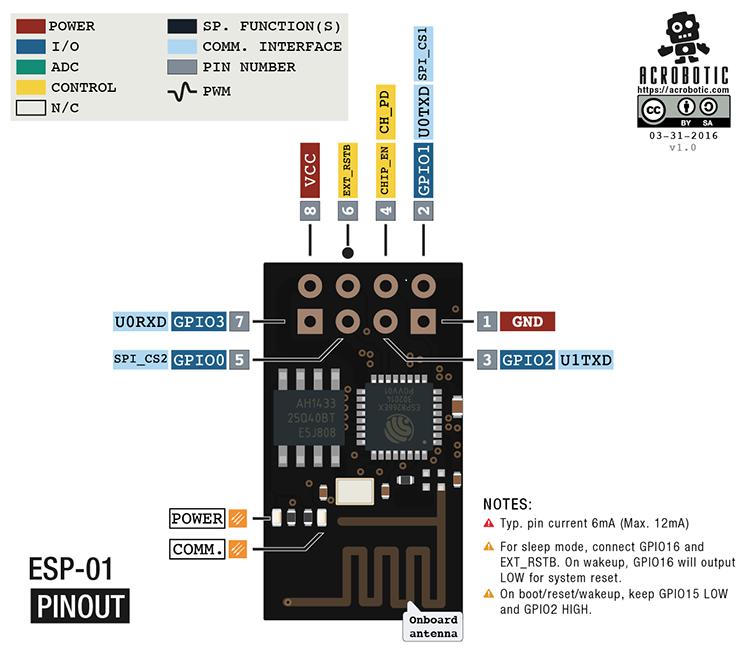
\includegraphics[width=10cm]{resources/pcb_res/esp8266_esp01_pinout.png}
            \caption{ESP-01 pinout-ja}
            \label{fig:eps01_pinout}
        \end{figure}
        
        A WS2811-es IC adatlapján a logikai jelszintes részt áttanulmányozva megállapítottam, hogy a mikrovezérlő 3,3V-os vezérlő jelét még éppen tolerálja a LED sor vezérlő IC 5V-os bemeneti lába (3,2V-os jel igaznak felel meg). 
        
        Ezek alapján állítottam össze a kapcsolást breadboard-on, és az internetről letöltött mintaprogramokat kicsit módosítva elértem, hogy külön-külön működött a Wifi modullal történő kommunikáció, illetve a LED soron meg tudtam jeleníteni egy fehér színt. Az összeállítással több probléma is volt: a tesztelés során a breadboardból gyakran kicsúsztak a kábelek, a csatlakozások kontaktosak voltak, hamis színeket okozva ezzel a LED soron. 
        
        A problémák orvoslásaként került sor a második fázis kivitelezésére, amit az Autodesk Eagle nyáktervező programmal valósítottam meg. (A Mikrovezérlők c. tantárgy keretében megtanultunk az Autodesk Eagle nevű nyáktervező program használatát.) Az internetről letöltöttem és beimportáltam az STM32F103C8T6 mikrovezérlő fejlesztői lapjának
        % https://os.mbed.com/users/hudakz/code/STM32F103C8T6_Hello/wiki/Homepage
        ,az ESP8266-os modul ESP-01-es 
        % forras esp libraryra
        típusának a könyvtárait. Létrehoztam egy saját könyvtárt is az Ebay-ről rendelt DC/DC modulnak. Ez a feszültségátalakító állítja elő a 12V-os tápfeszültségből a 3,3V-osat. Egy pár csatlakozó, állatpotjelző LED és ellenállás hozzáadása után összehuzaloztam a megfelelő elemeket. 
        
        \begin{figure}[h!]
            \centering
                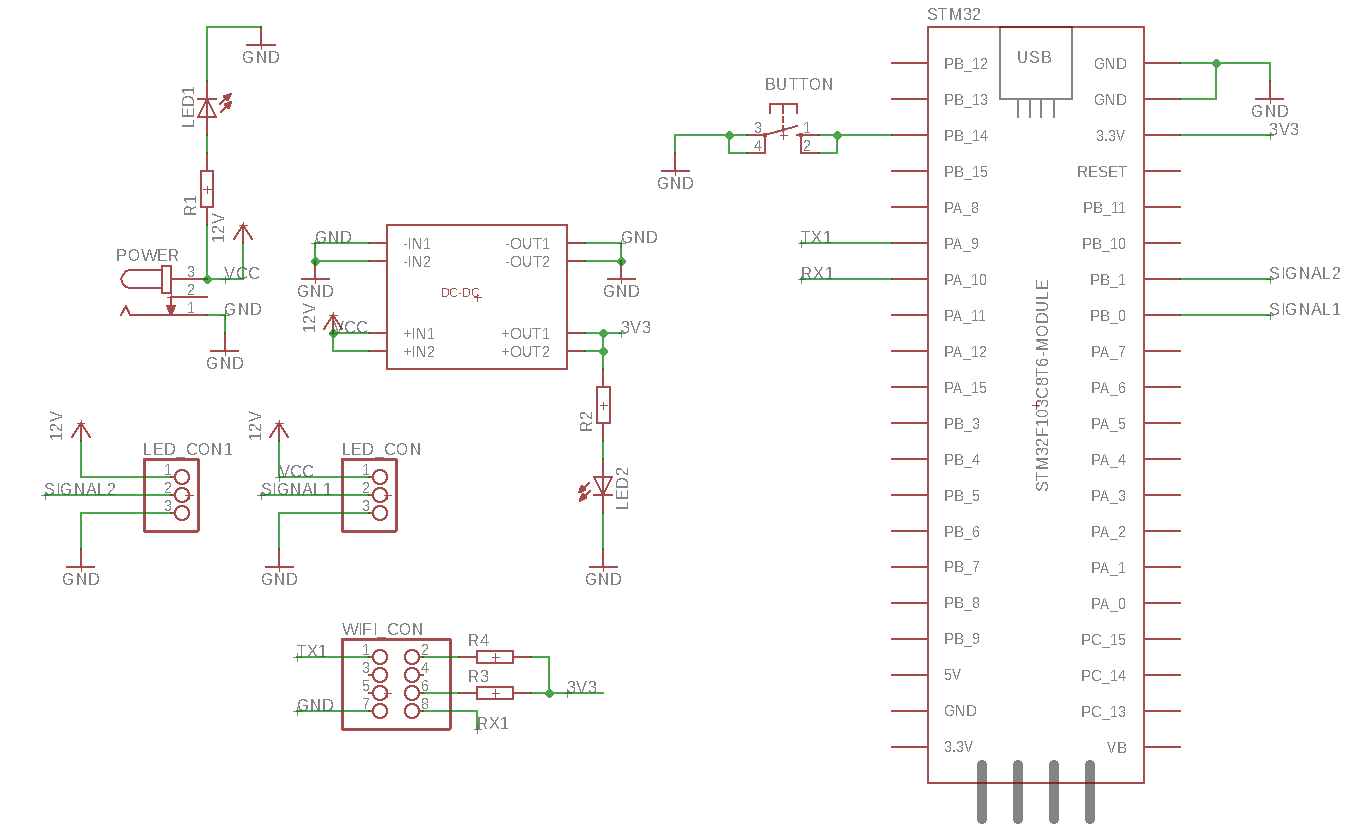
\includegraphics[width=15cm]{resources/pcb_res/schematic_v01.png}
            \caption{2. fázisú kapcsolási rajz}
            \label{fig:schematic_v01}
        \end{figure}
        
        Az elkészült kapcsolási rajz ( \ref{fig:schematic_v01}. ábra) alapján elhelyeztem és összekötöttem az alkatrészeket a NYÁK-on. Ezen a verzión bekötésre került egy extra gomb (BUTTON) és egy extra csatlakozó (LED\_CON1), hogy 2 LED sort legyen képes vezérelni az eszköz párhuzamosan. A \ref{fig:board_v01}. ábra szemlélteti az így összehuzalozott NYÁK-ot.
        
        \begin{figure}[h!]
            \centering
                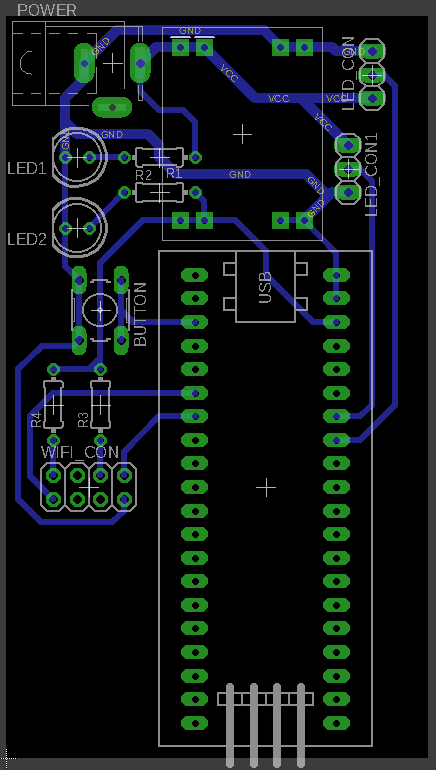
\includegraphics[width=5.5cm, angle =-90]{resources/pcb_res/board_v01.png}
            \caption{2. fázisú NYÁK-terv}
            \label{fig:board_v01}
        \end{figure}
        
        A NYÁK-ot vasalásos technikával készítettem el: a tervet lézernyomtatóval fényes papírra kinyomtattam, egy egy-oldalas NYÁK-lapra helyeztem, a tonerport vasalóval átvittem a rézfelületre, a tonerrel nem fedett réz bevonatú részeket maratószerrel lemarattam, és acetonnal lemostam, hogy a megmaradt rézfelületre forrasztani lehessen. Az így elkészült NYÁK-lapra (\ref{fig:pcb_v01}. ábra) beforrasztottam az alkatrészeket. Ezzel a NYÁK-kal már el tudtam kezdeni a beágyazott szoftver fejlesztését, mivel az elektronikai rész stabilan működött.
        
        \begin{figure}[h!]
            \centering
                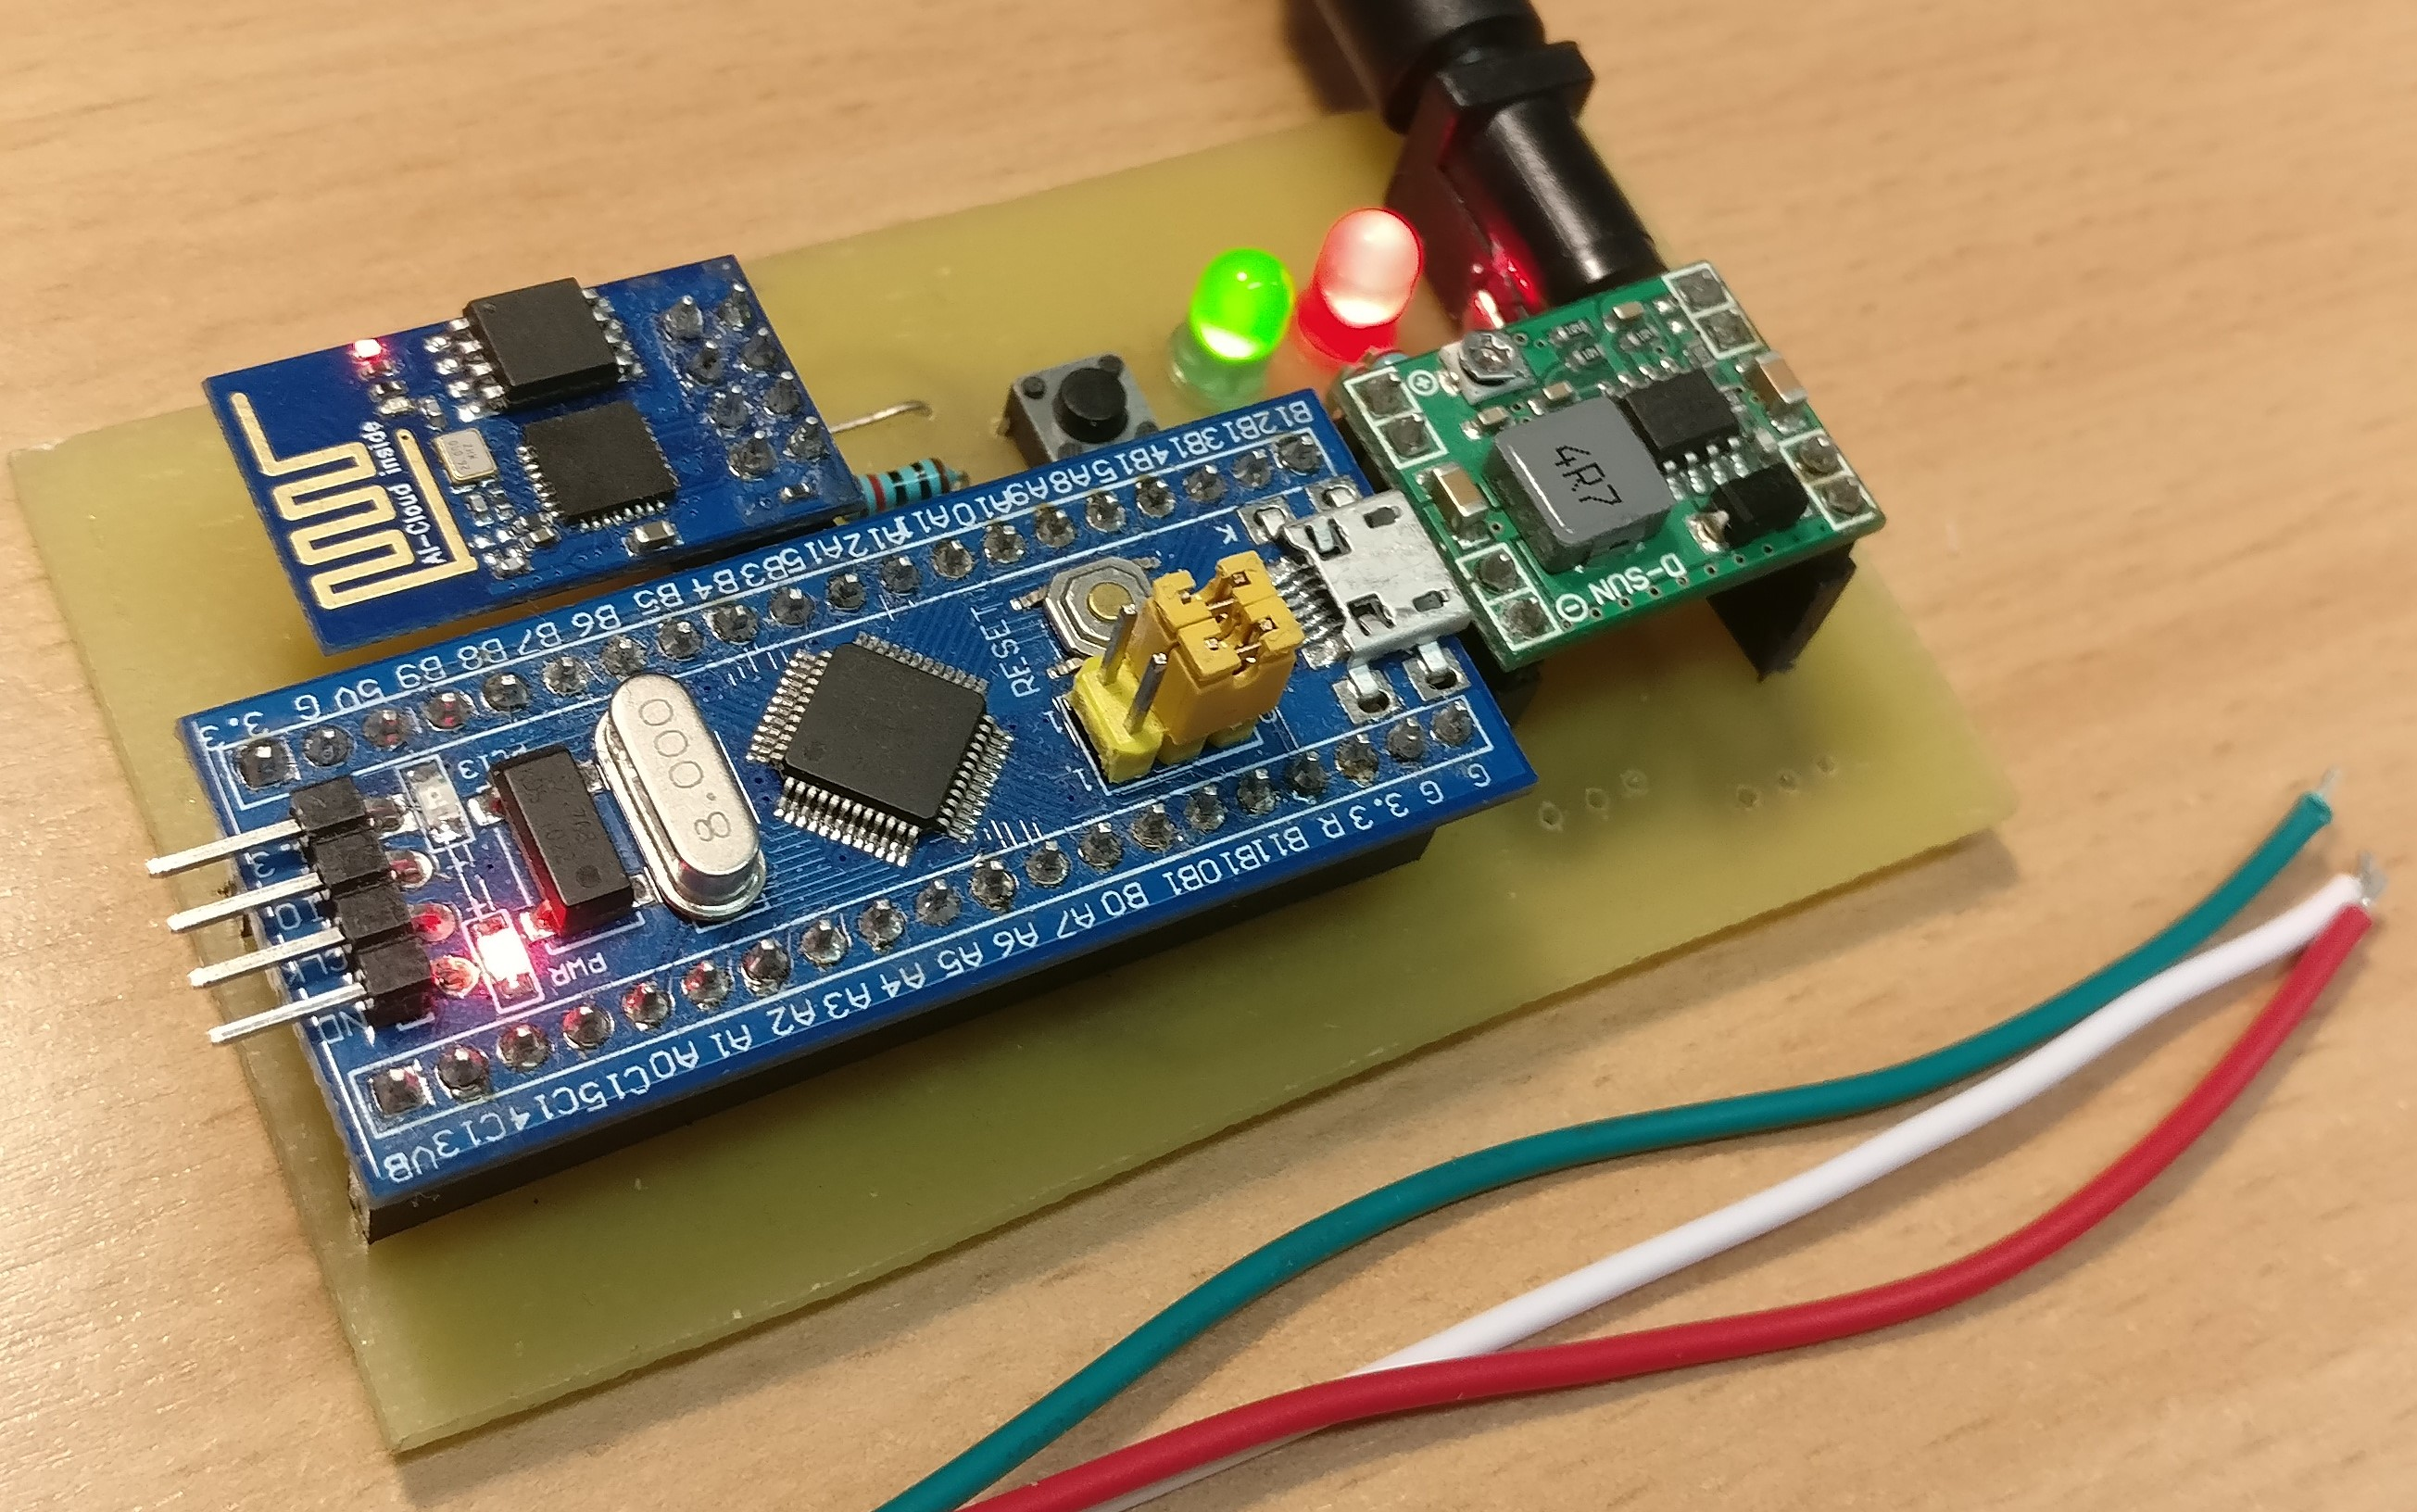
\includegraphics[height=4.5cm]{resources/pcb_res/pcb_v01}
                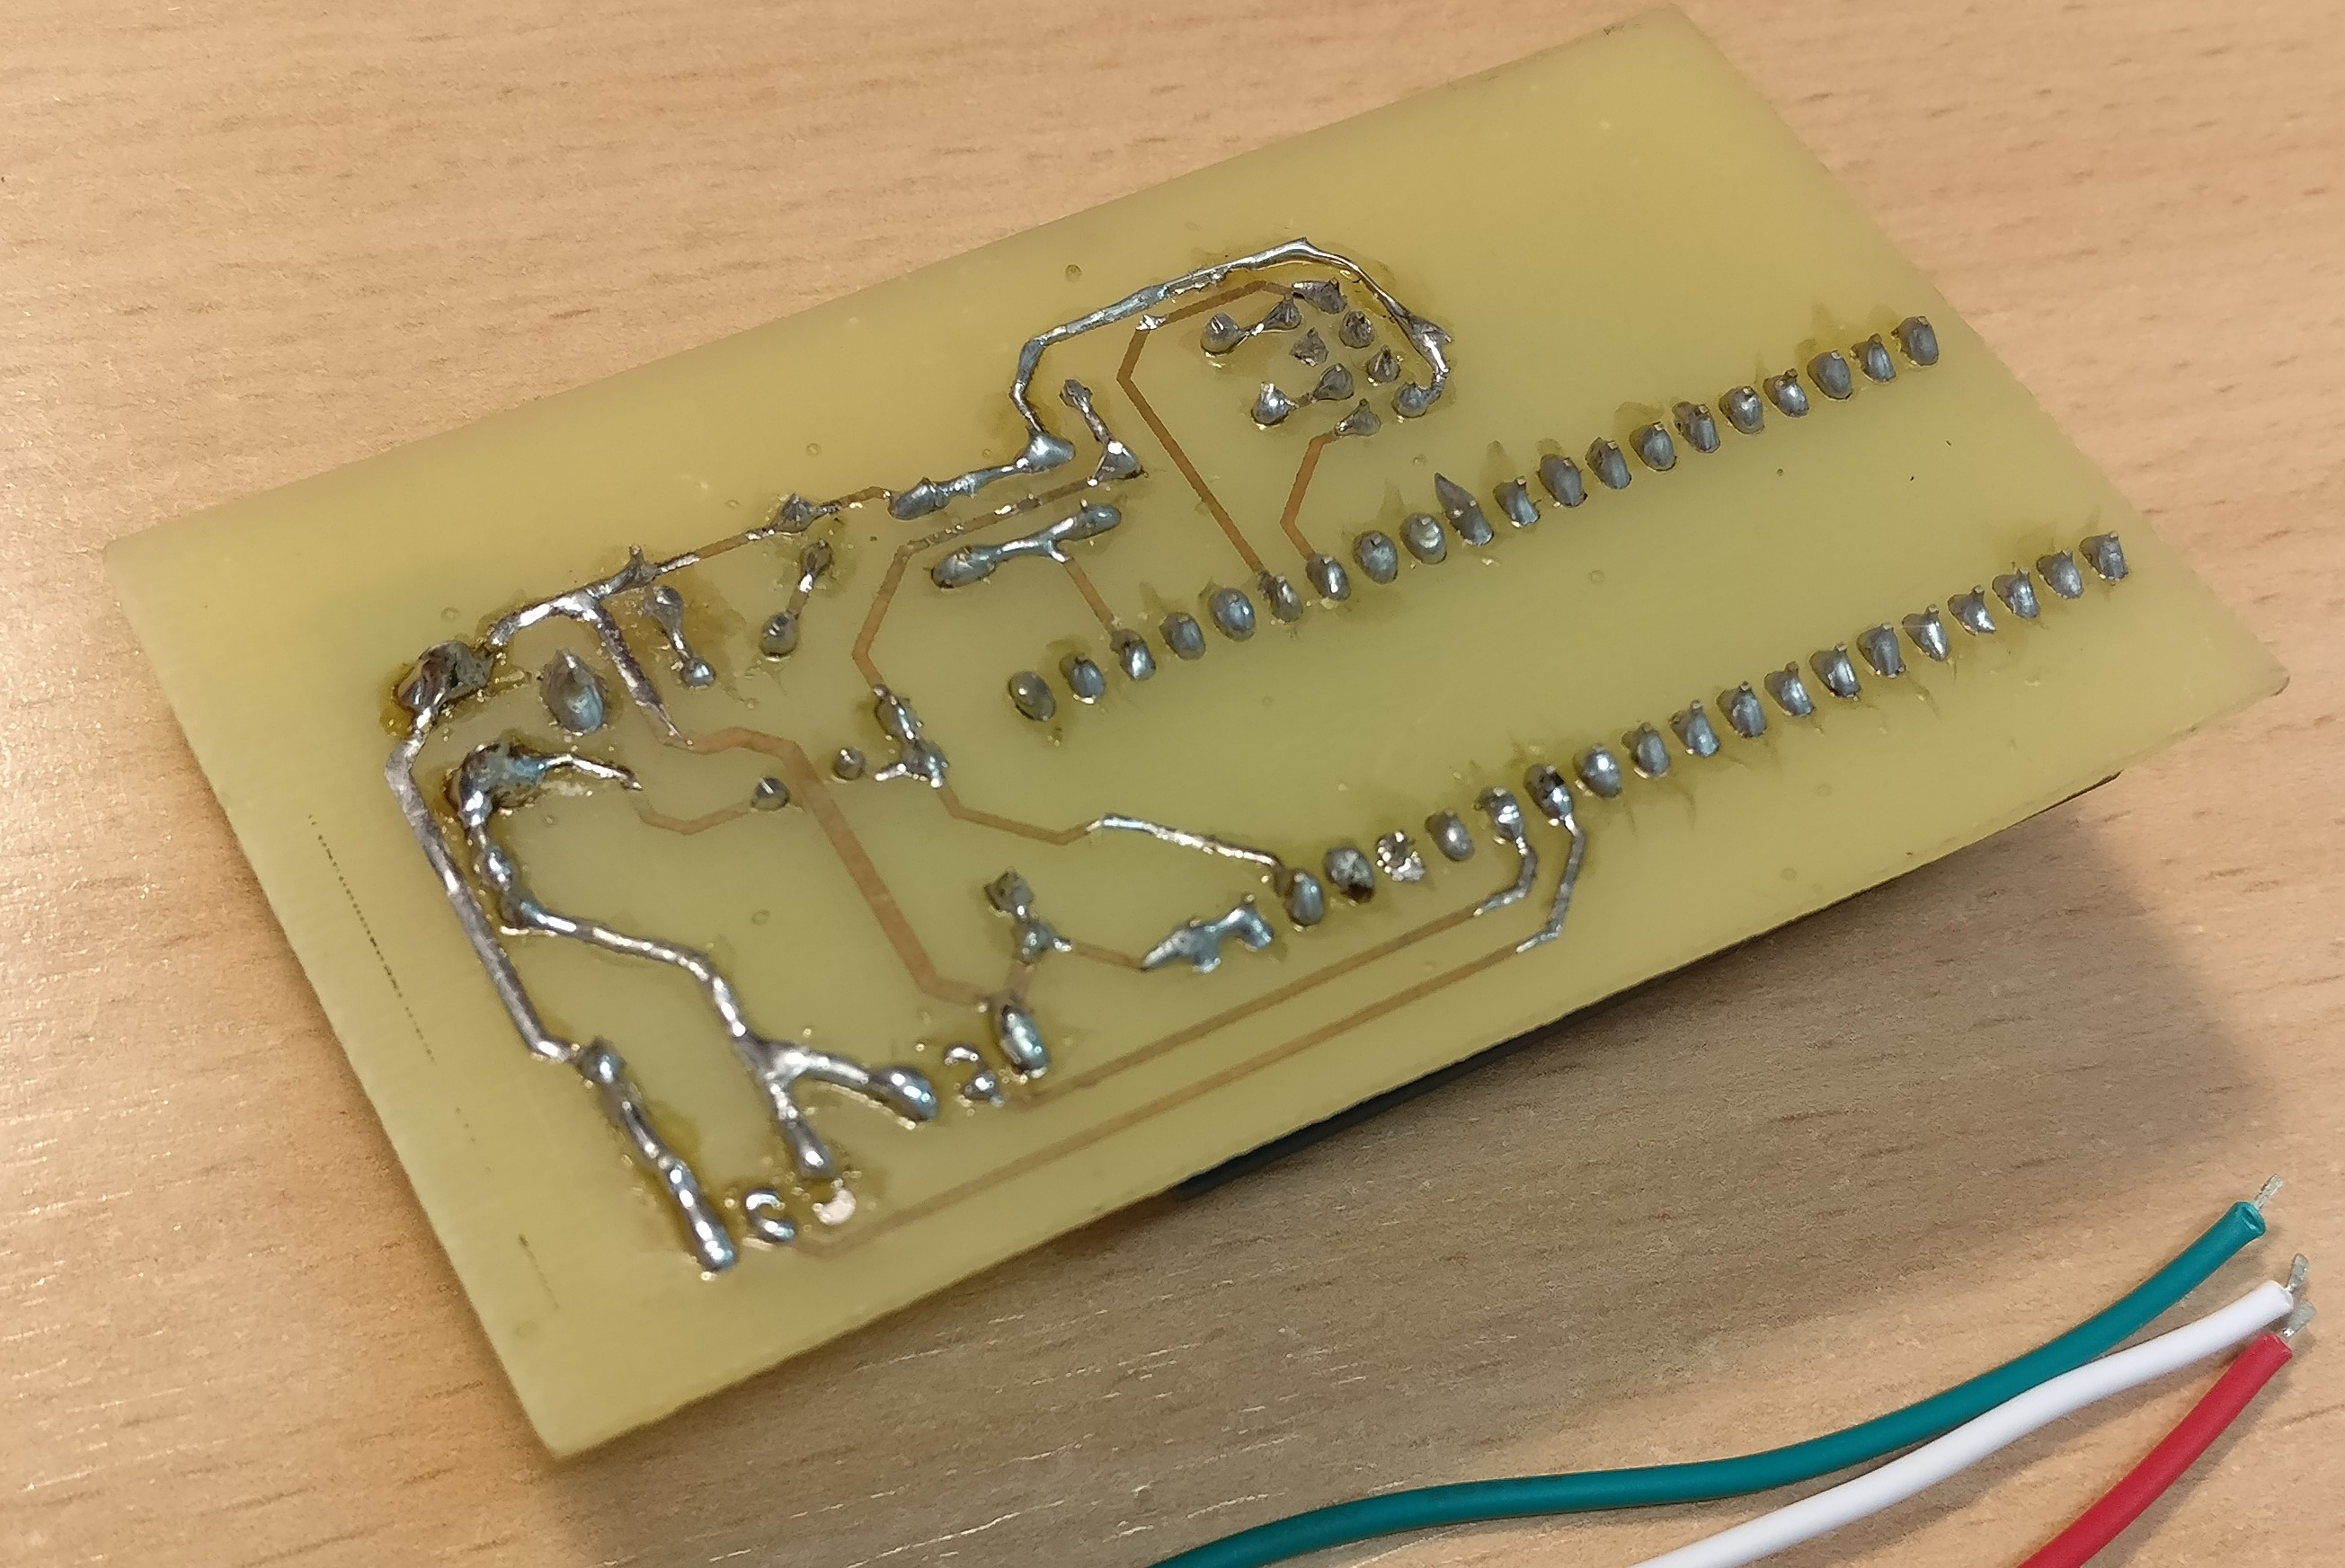
\includegraphics[height=4.5cm]{resources/pcb_res/pcb_v02}
            \caption{2. fázisú beforrasztott áramkör}
            \label{fig:pcb_v01}
        \end{figure}
        
        A 3. fázis tartalmazza DC/DC áramkörök tervezését és mikrovezérlő perifériáival együtti integrálását egy nyomtatott áramköri lapra.
        % a mondat második felét nem sikerül értelmeznem, hogy pontosan mit szeretnél vele de ezt át kéne fogalmazni olyasmire h a 3. fázis ... és ...-ból áll. (Betti)
        
        \subsubsection{DC/DC tervezés}
            %https://www.quora.com/Where-can-I-use-LDO-and-DC-DC-converters
            Mivel nagy a különbség a bemeneti és kimenteti feszültségek között (12V-ról 5V-ra), ezért egy DC/DC konverter sokkal jobban megfelel, mint egy LDO (Low-DropOut regulator), hiszen egy LDO-nak a hatékonysága nagyon alacsony (12V-ról 5V-ra kb. 41\%) és a maradék energiát elfűti. Ez a megoldás semmiképpen sem előnyös, illetve még hűtőborda alkalmazását is megköveteli.
            
            %https://electronics.stackexchange.com/questions/160218/how-does-dcdc-save-power-over-an-ldo
            % zajos 
            % nehezebb a tervezes
            % több komponensből áll
            
            A 3,3V és 5V-os tápfeszültségek ellőállítására 2 DC/DC áramkörre is szükségem volt, és ezért olyan megoldást kerestem, ahol ez ugyanazzal az IC-vel, külső komponensek minimális változtatásával ez megoldható. Célom volt továbbá, hogy egy 3 cellás LiPo akkumulátorról is működjön az áramkör, ezáltal hordozható legyen. A bemeneti feszültség, 3V-os minimum és 4,2V-os maximum cella feszültségnél, egy 3 cellás LiPo-nál 9V és 12,6V közzé fog esni. A felső értéket egészre kerekítve és eggyel nagyobbra választva (14V) egy kisebb biztonsági sávot is kaptam.
            \\
            A DC/DC áramkörök tervezésénél nagy segítségemre volt a TI (Texas Instruments) Webench Power Designer.
            % https://webench.ti.com/webench5/power/
            A tervezési paramétereket megadva nem csak egy megfelelő IC-t, hanem több komplett kapcsolást is felkínál. A kimeneti névleges áramot, a 3,3V-os kimeneti feszültség esetében, 1,5A-ra választottam (\ref{fig:ti_we_des_param_3v3}. ábra), hogy akár még más áramköri lapkát is képes legyen meghajtani az eszköz. Az 5V-os kimenet esetén (\ref{fig:ti_we_des_param_5v}. ábra) is túlméreteztem a névleges áramot (0,5A).
            % esp8266 datasheet
            % https://www.espressif.com/sites/default/files/documentation/0a-esp8266ex_datasheet_en.pdf 
            \begin{figure}[h!] % https://webench.ti.com/webench5/power/
                \begin{floatrow}
                    \ffigbox{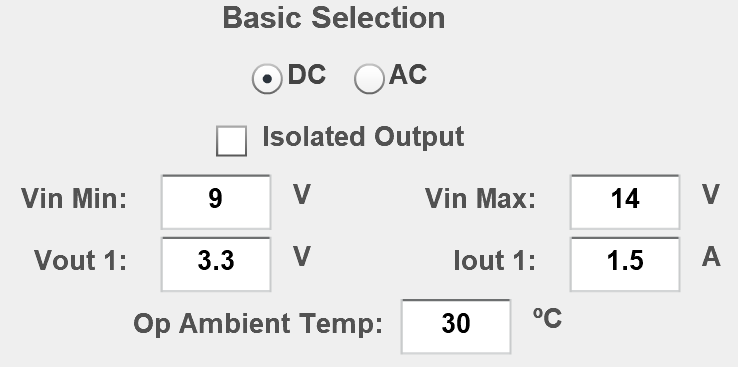
\includegraphics[width=7cm]{resources/pcb_res/ti_we_des_param_3v3.png}}{\caption{Tervezési paraméterek megadása 3,3V-os kimentre}\label{fig:ti_we_des_param_3v3}}
                    \ffigbox{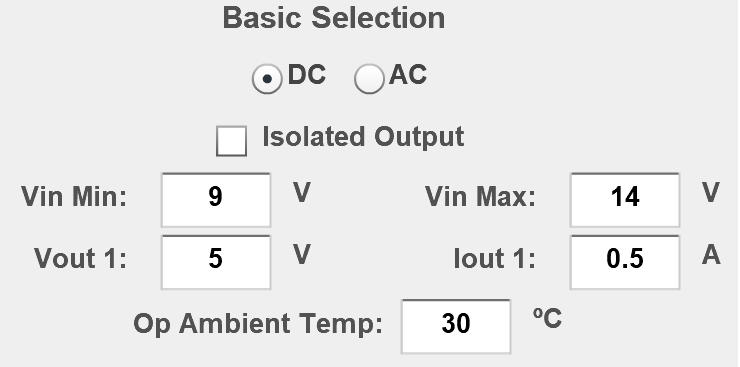
\includegraphics[width=7cm]{resources/pcb_res/ti_we_des_param_5v.png}}{\caption{Tervezési paraméterek megadása 5V-os kimentre}\label{fig:ti_we_des_param_5v}}
                \end{floatrow}
            \end{figure}
            
            Ezek után az integrált, könnyen használható és költséghatékony módszert választva (\ref{fig:ti_we_des_int_etu_ce_method}. ábra) elkezdtem keresgélni a legenerált esetek között, minél olcsóbb és hatékonyabb megoldást keresve. % nem érthető ez a mondat (Betti)
            
            \begin{figure}[h!]
                \centering
                    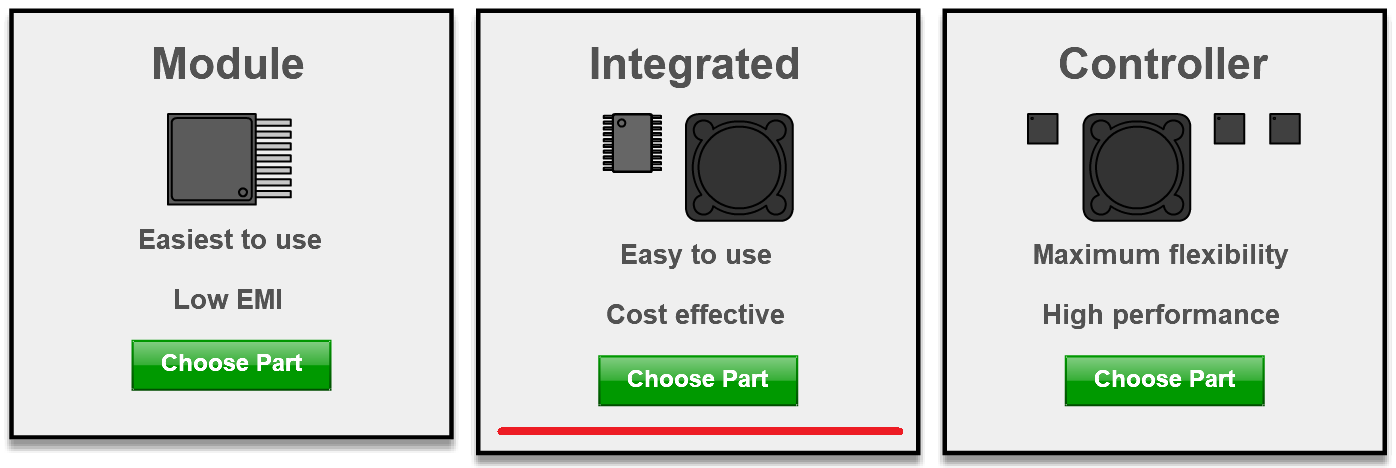
\includegraphics[width=10cm]{resources/pcb_res/ti_we_des_int_etu_ce_method_2.png}
                \caption{Tervezési séma kiválasztása}
                \label{fig:ti_we_des_int_etu_ce_method}
            \end{figure}
            
            A TPS562219A típusú IC mindkét konfigurációban (3,3V - 5V) előfordult. A két verzió között %(3,3V - 5V) 
            csak egy tekercs és egy ellenállás volt a különbség.
            
            A TI Webench Designer által kínált kapcsolási rajzok komponensei nem mindig megfelelőek, illetve beszerezhetőek. (Tovább bonyolította helyzetet, hogy SMD komponenseket sohasem forrasztottam, tehát az alkatrészek mérete sem volt mindegy számomra.) A korábbi tapasztalataim alapján úgy döntöttem hogy 1206-os (metrikus: 3216) SMD méretet fogok használni. Az egyik legnagyobb elektronikai kereskedőnél, a Mouser Electronics-nál, a megfelelő paraméterek figyelembevételével újraválasztottam az alkatrészeket. Miután néhány komponensnek megcsináltam az Eagle könyvtárát, elkészítettem a kapcsolási rajzokat a Webench Designer és a TPS562219A IC adatlapja alapján. Mivel a két konfiguráció (3,3V - 5V) minimálisan különbözik egymástól ezért csak az egyiket ábrázoltam (\ref{fig:schematic_3v3}. ábra).
            
            \begin{figure}[h!]
                \centering
                    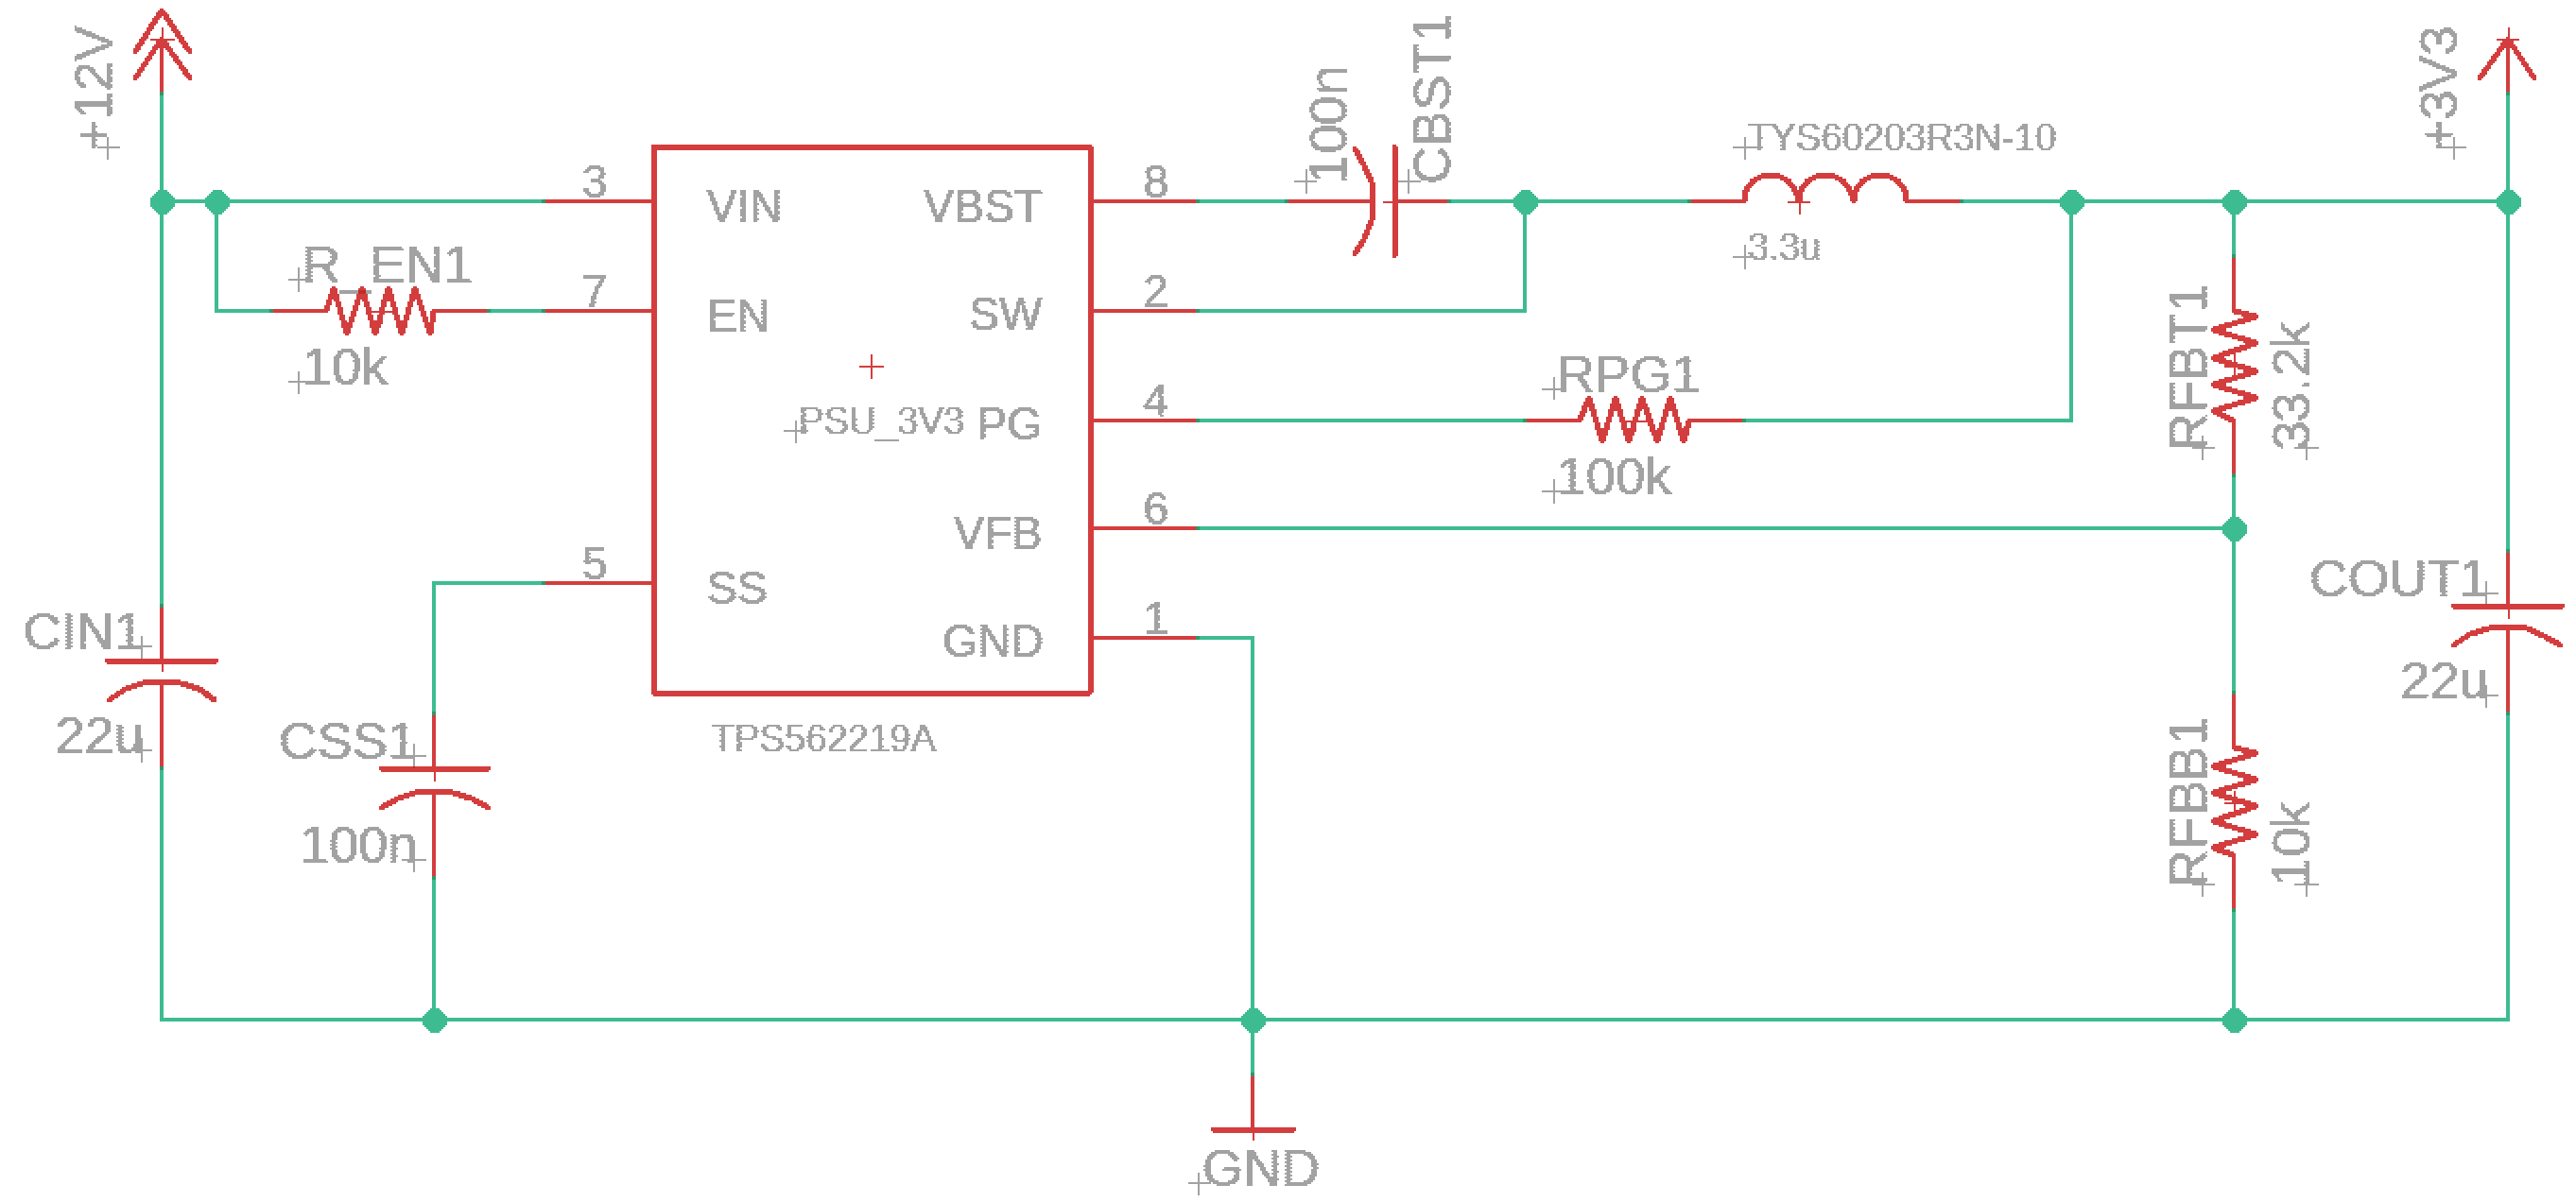
\includegraphics[width=12cm]{resources/pcb_res/schematic_3v3.png}
                \caption{3,3V-os DC/DC kapcsolási rajza}
                \label{fig:schematic_3v3}
            \end{figure}
            
            Általáben nem mindegy, hogy az alkatrészeinket az adott IC körül milyen kiosztásban helyezzük el. A TPS562219A típusú IC adatlapjában pontokba van szedve mire kell odafigyelni, illetve egy elhelyezési minta (\ref{fig:tps_logl_example}. ábra) is megtalálható mellette.
            % irányelvek resz
            
            \begin{figure}[h!]
                \centering
                    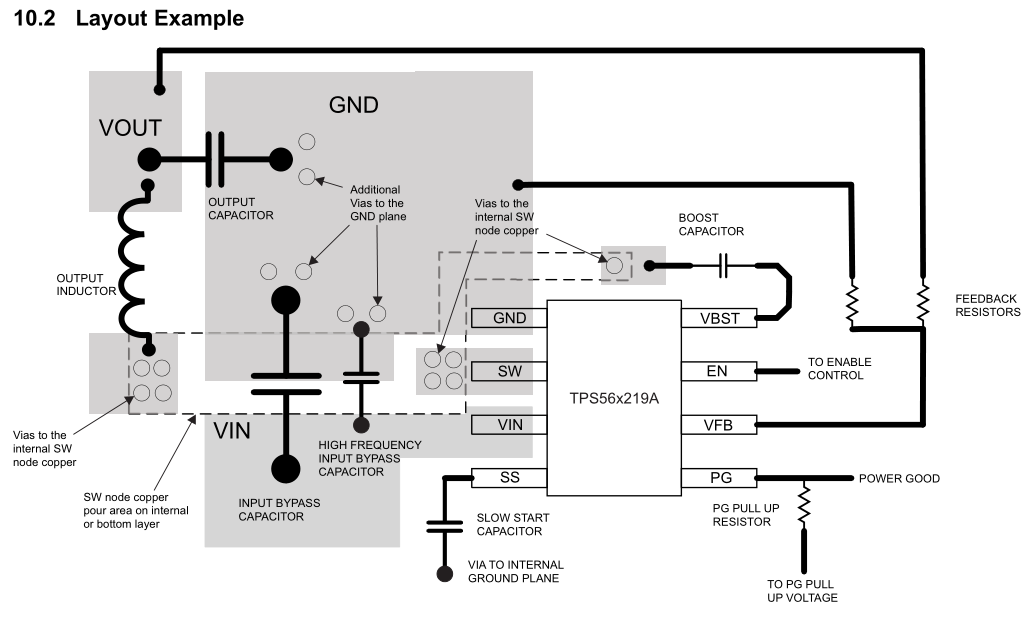
\includegraphics[width=12cm]{resources/pcb_res/tps_logl_example.png}
                \caption{DC/DC elhelyezési mintája}
                \label{fig:tps_logl_example}
            \end{figure}
            
            Az irányelveket követve az elkészült NYÁK-tervet \aref{fig:pcb_3v3}. ábra szemlélteti.
            
            \begin{figure}[h!]
                \centering
                    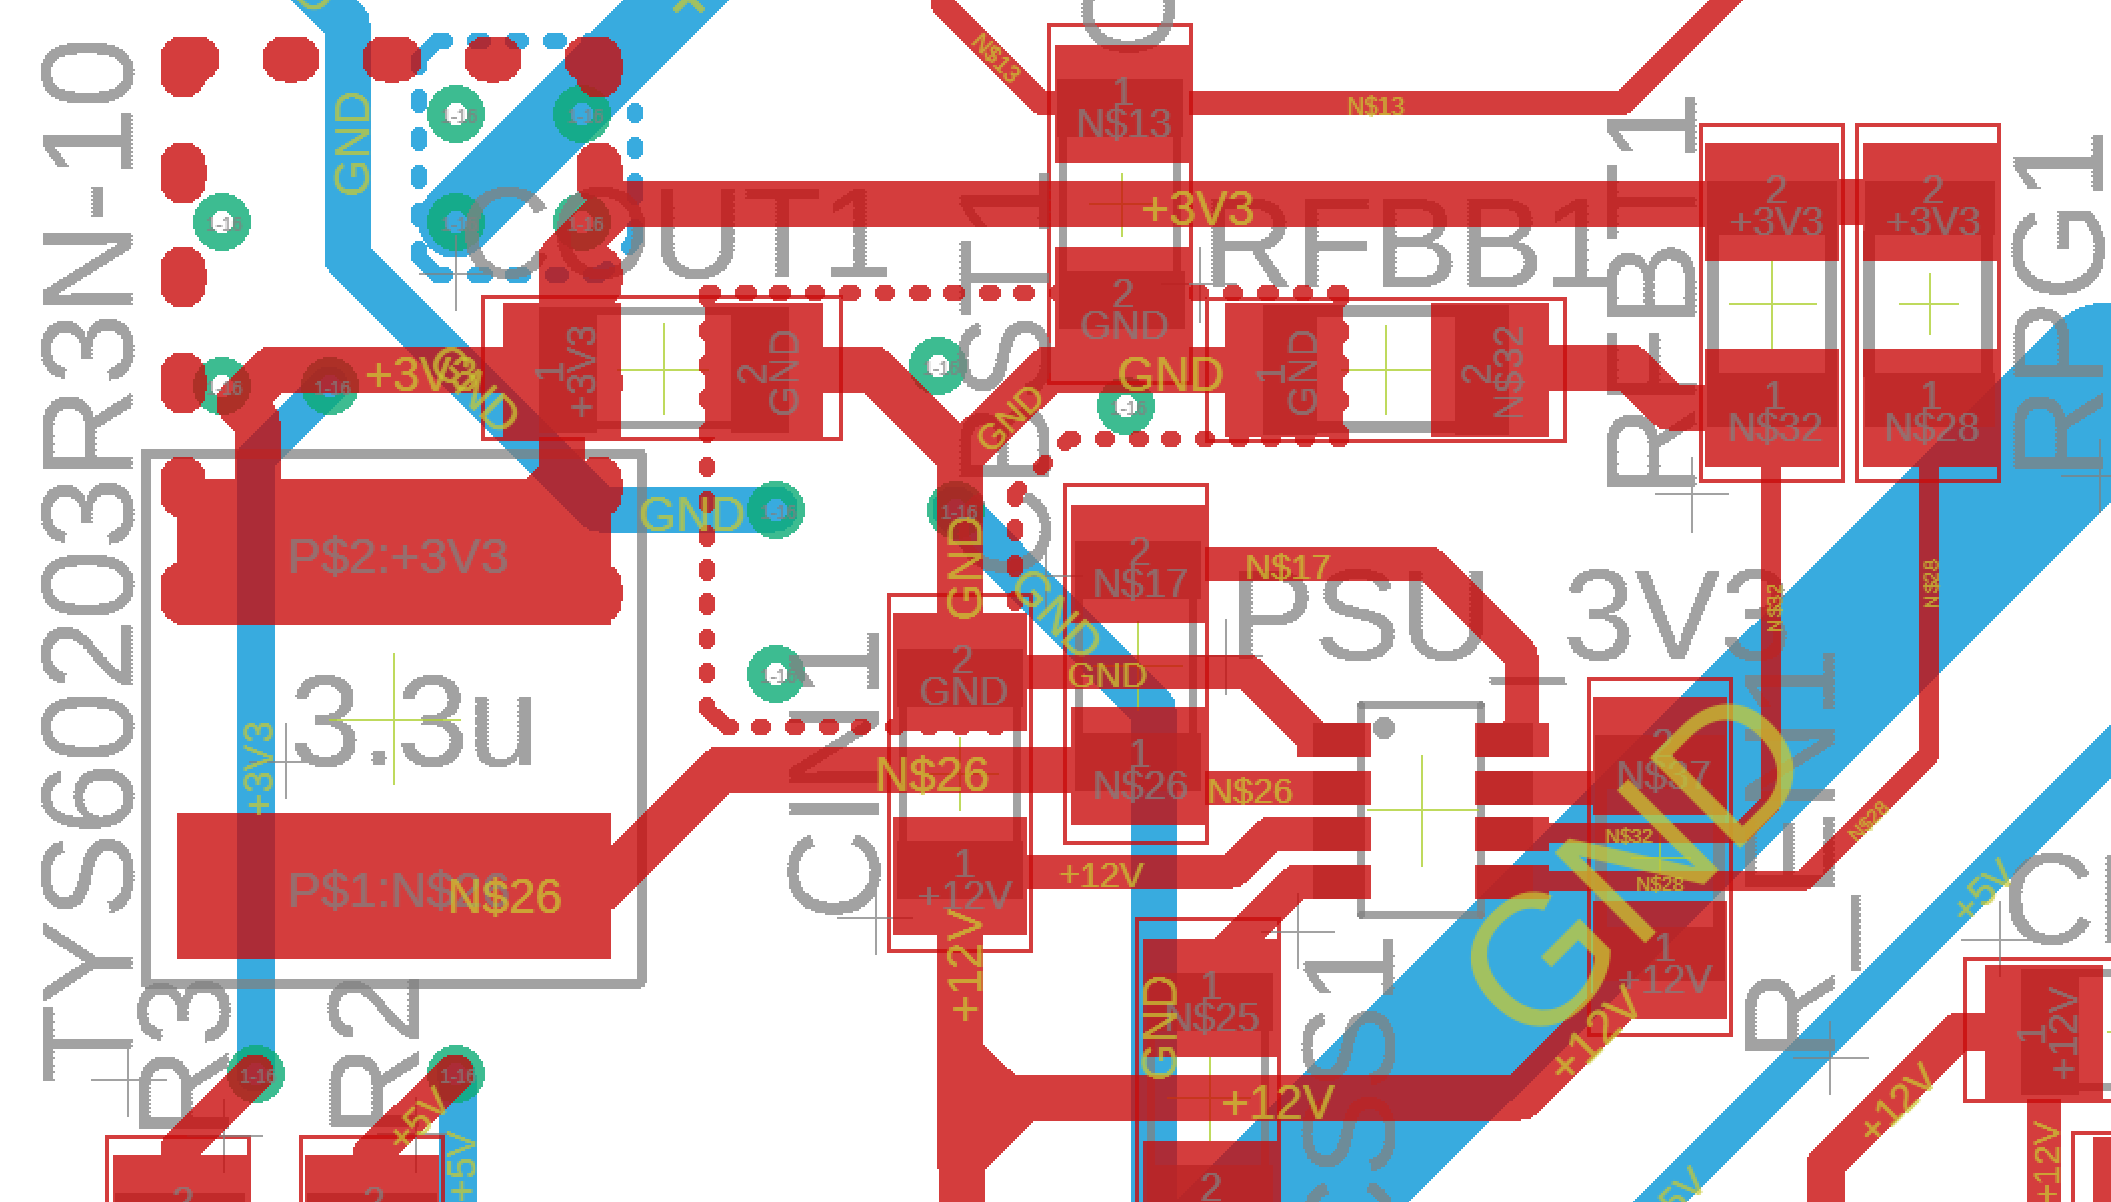
\includegraphics[width=6.5cm]{resources/pcb_res/board_dcdc_3v3.png}
                    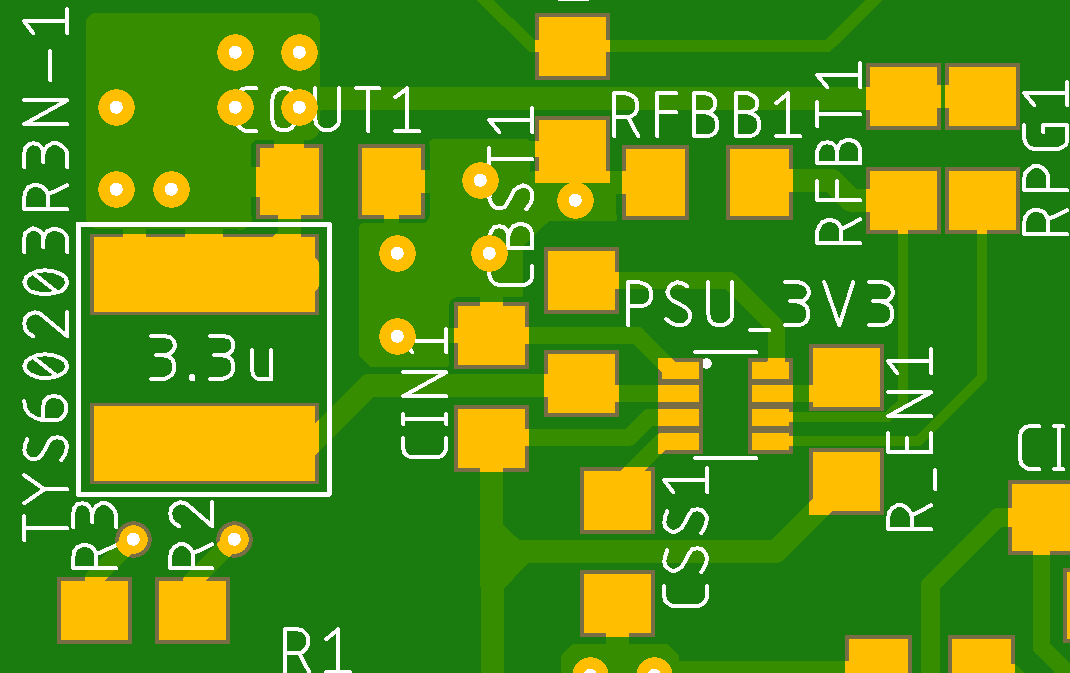
\includegraphics[width=6cm]{resources/pcb_res/pcb_dcdc_3v3.png}
                \caption{3,3V-os DC/DC nyákterve}
                \label{fig:pcb_3v3}
            \end{figure}
            
            Hasonló módon készíttettem el az 5V-os átalakítót is, csak az a rész NYÁK-on az óra mutató járásával megegyezően 90°-al el lett forgatva.
            
        \subsubsection{Logikai jelszint átalakító tervezése}
            A WS2811-es IC adatlapjában (//TODO - forrasmegjeloles) le van írva, hogy a tápfeszültség (V$_DD = 4,5..5,5V$) 70\%-nak kell lennie a vezérlő jelnek, hogy az IC logikai 1-es szintnek értelmezze. Tehát minimum 3,15V-os ($0,7\cdot4,5V=3,15V$) jel kell az IC vezérléséhez. Így a 3,3V-os mikrovezérlővel a határon mozgok és feszültségingadozás esetén zavarok léphetnek fel. A megbízható, stabil működéshez egy logikai jelszint átalakítót kell beépítenem az áramkörbe. 

            Törekedtem minél több alkatrészt a TI-től (Texas Instruments) kiválasztani, mert a diákok (érvényes egyetemi e-mail-címmel rendelkezők) számára egy pár ingyenes mintadarabot kínál, amikkel jobb esetben elvégezhető a prototípus fejlesztése. Így esett a választásom a SN74LV1T34 típusú logikai jelszint átalakítóra.
            
            \begin{figure}[h!]
                \begin{floatrow}
                    \ffigbox{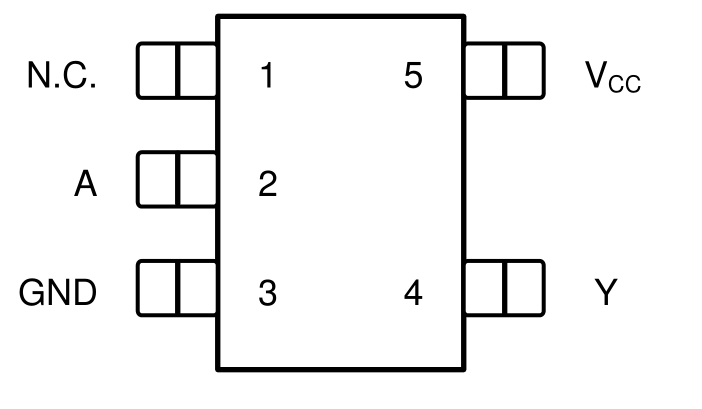
\includegraphics[width=5cm]{resources/pcb_res/SN74LV1T34_pinout.png}}{\caption{SN74LV1T34 logikai jelszint átalakító IC lábkiosztása}\label{fig:SN74LV1T34_pinout}}
                    \ffigbox{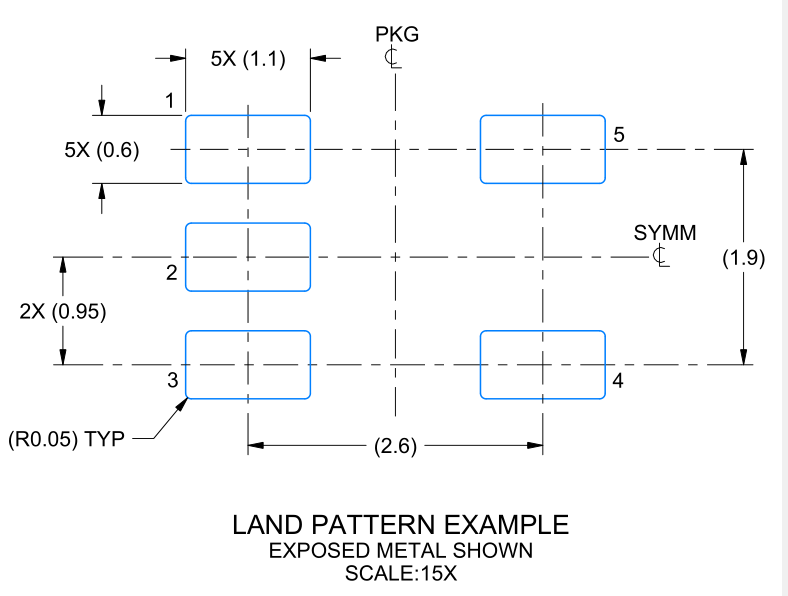
\includegraphics[width=5cm]{resources/pcb_res/SN74LV1T34_land_pattern.png}}{\caption{SN74LV1T34 IC padjeinek elhelyezkedése}\label{fig:SN74LV1T34_land_pattern}}
                \end{floatrow}
            \end{figure}
            
            
            A kis SOT-23-as csomagolású IC (\ref{fig:SN74LV1T34_pinout}. ábra) rendkívül egyszerűvé tette a feladatomat. A 'GND' lábára a földet , az 'A' lábára a bemeneti jelet, az 'Y' lábára a kimeneti jelet, a 'V$_{cc}$' lábára pedig a kívánt kimeneti logikai jelszintnek megfelelő 5V tápfeszültséget %kellett kötnöm.
            kötöttem. Az adatlapban leírt forrasztási maszk (\ref{fig:SN74LV1T34_land_pattern}. ábra) alapján elkészíttettem az alkatrész Eagle könyvtárát. A 3. fázisú NYÁK-kal már három LED sort szerettem volna vezérelni, ezért a kapcsolási rajzon és a nyákon is három-három darab alkatrész került elhelyezésre.
            
            // képek?? kell/nem? %az elejére kéne valami kis összefoglaló mondat arról hogy a különböző fázisú nyákokkal mi a cél (Betti)
        
        \subsubsection{STMF103C8T6 mikrokontroller és perifériák}
            A mikrokontrollert külső komponensekkel is el kell látni ahhoz, hogy megfelelően működjön. Az első és legfontosabbak a bufferkondenzátorok a mikrokontroller megfelelő lábain. Az alkalmazási útmutató (//TODO application note (an2586) - getting started with stm32f103) leírja, hogyan kell a kondenzátorokat megfelelően bekötni őket (\ref{fig:decoupling_cap}. ábra): minél közelebb a megfelelő lábakhoz, és ha lehetséges akkor átviázva//TODO - ezt hogy mondom magyarul?// a föld ($V_{SS}$) és a tápfeszültség ($V_{DD}$) rétegekre. Az adatlapban (\ref{fig:decoupling_cap}. Ábra) pedig megtalálható, hogy melyik lábra mekkora és milyen kondenzátort kell bekötni.
            
            \begin{figure}[h!]
                \centering
                    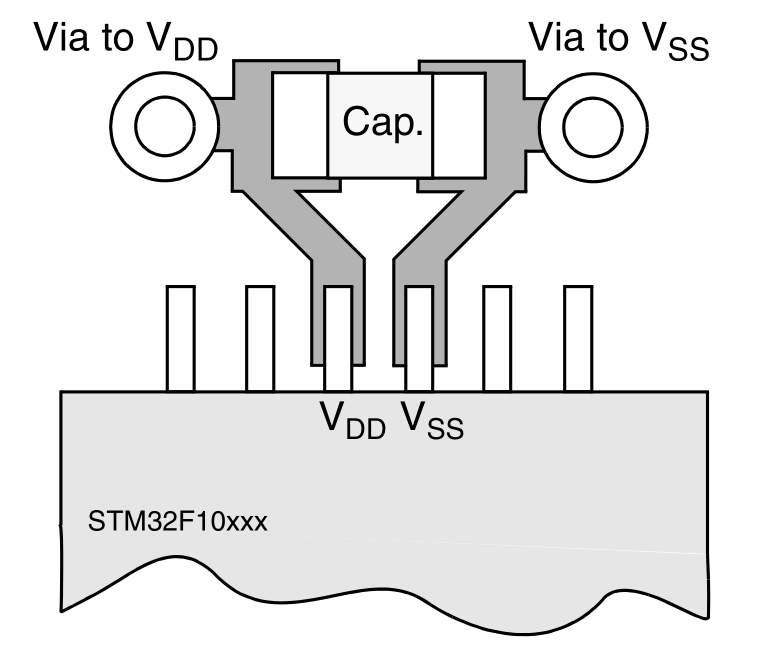
\includegraphics[width=4.5cm]{resources/pcb_res/decoup_cap.png}
                    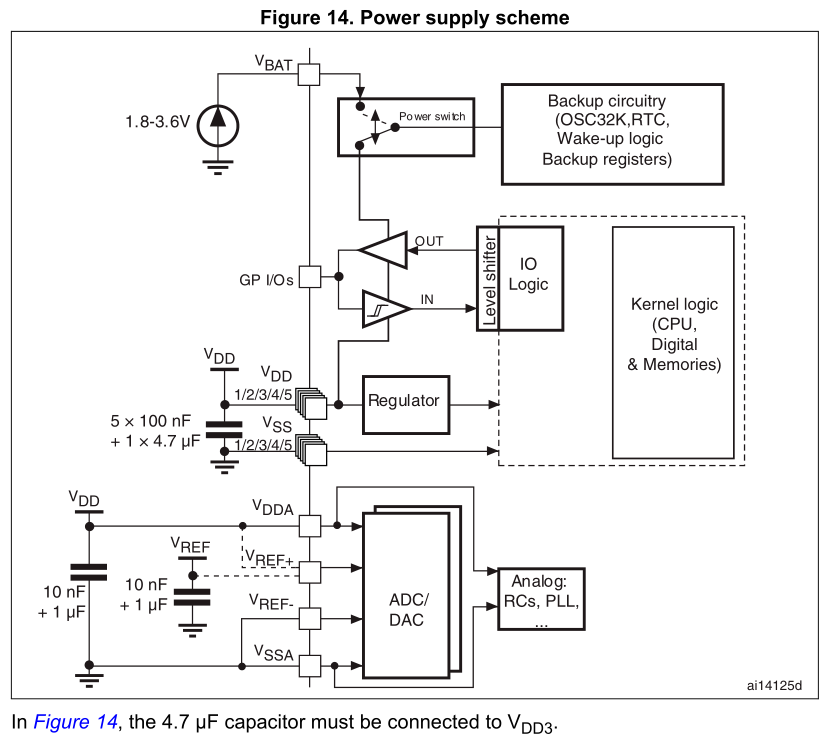
\includegraphics[width=10.5cm]{resources/pcb_res/power_sup_capacitors.png}
                \caption{Bufferkondezátorok ajánlott áramköri elhelyezése balra, méreteik, bekötési helyeik jobbra}
                \label{fig:decoupling_cap}
            \end{figure}
            
            % \begin{figure}[h!]
            %     \begin{floatrow}
            %         \ffigbox{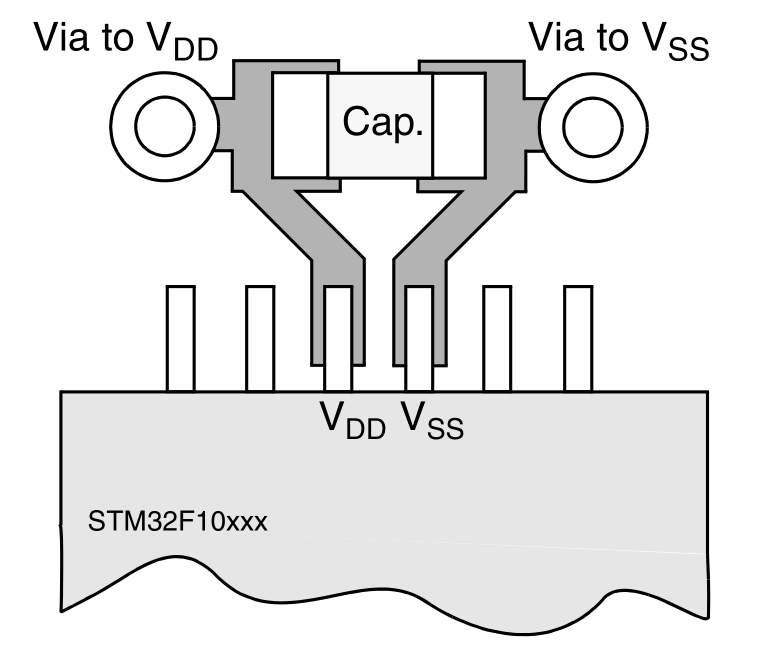
\includegraphics[width=4cm]{resources/pcb_res/decoup_cap.png}}{\caption{Bufferkondezátor ajánlott áramköri elhelyezése}\label{fig:decoupling_cap}}
            %         \ffigbox{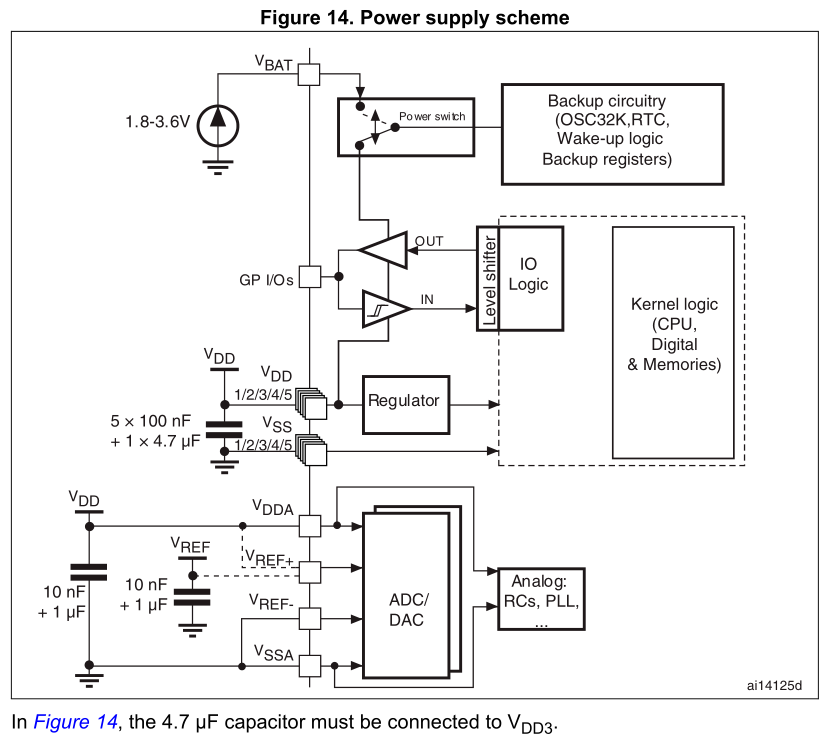
\includegraphics[width=8cm]{resources/pcb_res/power_sup_capacitors.png}}{\caption{Bufferkondenzátorok méretei és bekötési helyei}\label{fig:power_sup_capacitors}}
            %     \end{floatrow}
            % \end{figure}
            
            Többféle képpen is felprogramozható (UART-on keresztül bootloader segítségével, JTAG-en vagy pedig SWD-n) a mikrokontroller, viszont DEBUG-olni csak JTAG-en és SWD-n (Serial Wire Debug) lehet. A kettő közül az utóbbit választottam, mert rendelkezésemre állt egy USB-s SWD programozó. Ahhoz, hogy a mikrokontrollert SWD-n keresztül programozhassuk, ki kell vezetni a SWCLK (Serial Wire Clock), illetve SWDIO lábakat egy csatlakozóra. A kétirányú kommunikáció miatt (programozás, debuggolás), az SWDIO vezetéket egy 100[k$\Omega$]-os ellenállással ajánlott felhúzni a tápfeszültségre (//TODO ref - reference manual (RM0008) 31.8.1-es section). 
            
            //TODO boot pinek kimaradtak
            
            A maximális, 72MHz-es, órajellel való működéshez külső oszcillátor áramkörre is szükség van, anélkül csak 64MHz lenne elérhető. A referencia terv (\ref{fig:hse_ref_des}. ábra) alapján egy 8MHz-es kristály oszcillátort és két 20pF-os kerámiakondenzátort használtam a megvalósításhoz. 
            
            \begin{figure}[h!]
                \centering
                    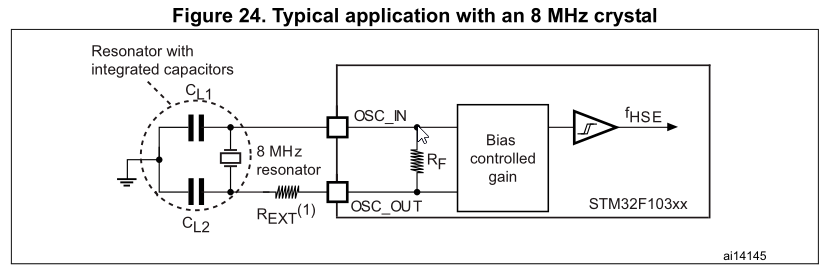
\includegraphics[width=12cm]{resources/pcb_res/hse_ref_des.png}
                \caption{Nagy sebességű oszcillátor referencia terv}
                \label{fig:hse_ref_des}
            \end{figure}
            
            A reset gombot is bekötöttem, szintén csak az adatlap által javasolt referencia terv (\ref{fig:reset_ref_des}. ábra) alapján.
            
            \begin{figure}[h!]
                \centering
                    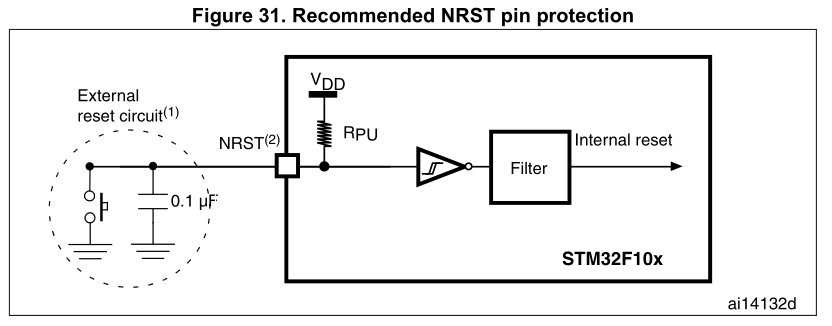
\includegraphics[width=12cm]{resources/pcb_res/reset_ref_des.png}
                \caption{Reset gomb bekötésének referencia terve}
                \label{fig:reset_ref_des}
            \end{figure}
            
            A mikrokontrollert összekötöttem a Wifi modullal, illetve további 3 LED-es állapotjelző kimenettel és 3 szoftveresen földre húzott gombbal is elláttam a kapcsolást. Csak az egyik LED-nek szántam szerepet, a többi I/O továbbfejlesztési lehetőségnek lett megtervezve.
            
            Az ST Microelectronics gyártó STM32CubeMX nevű programjával ellenőriztem a megfelelő lábkiosztást, hogy a megfelelő lábakra kivezethetők-e az adott belső perifériák (TIMER-ek, UART) jelei. 
            \begin{figure}[h!]
                \centering
                    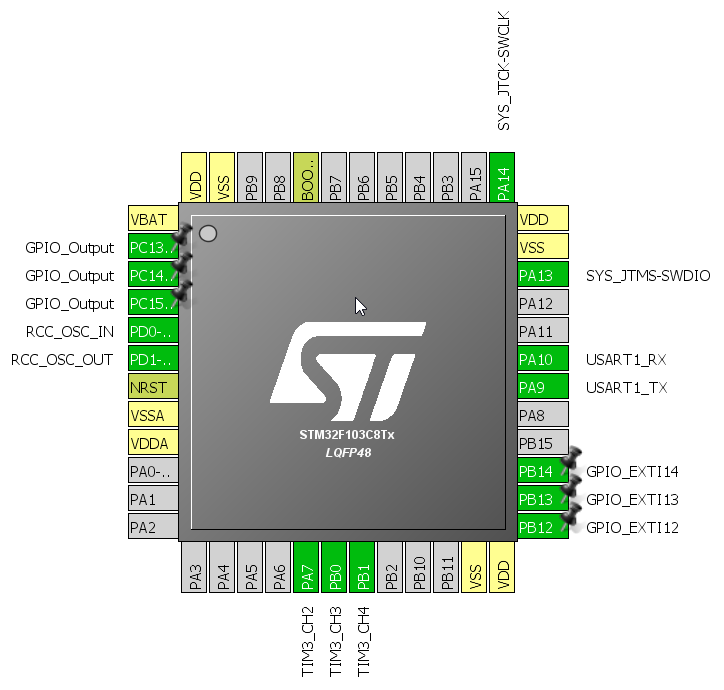
\includegraphics[width=8cm]{resources/pcb_res/cubeMX_pinout.png}
                \caption{Lábkiosztás a STM32CubeMX programban}
                \label{fig:CubeMX_pinout}
            \end{figure}
            
            
            A mikrokontrollerem EAGLE könyvtárát az internetről letöltöttem és beimportáltam a programba. A tervek alapján elkészítettem a kapcsolási rajzot (//TODO ref fuggelekbe ábra) pár extra visszajelző komponensel ellátva: UART RX, TX jelvezetékeire, a 12V-os és a DC/DC áramkörök kimenteti tápfeszültségeire kötöttem visszajelző LED-eket. 
            
            \begin{figure}[h!]
                \centering
                    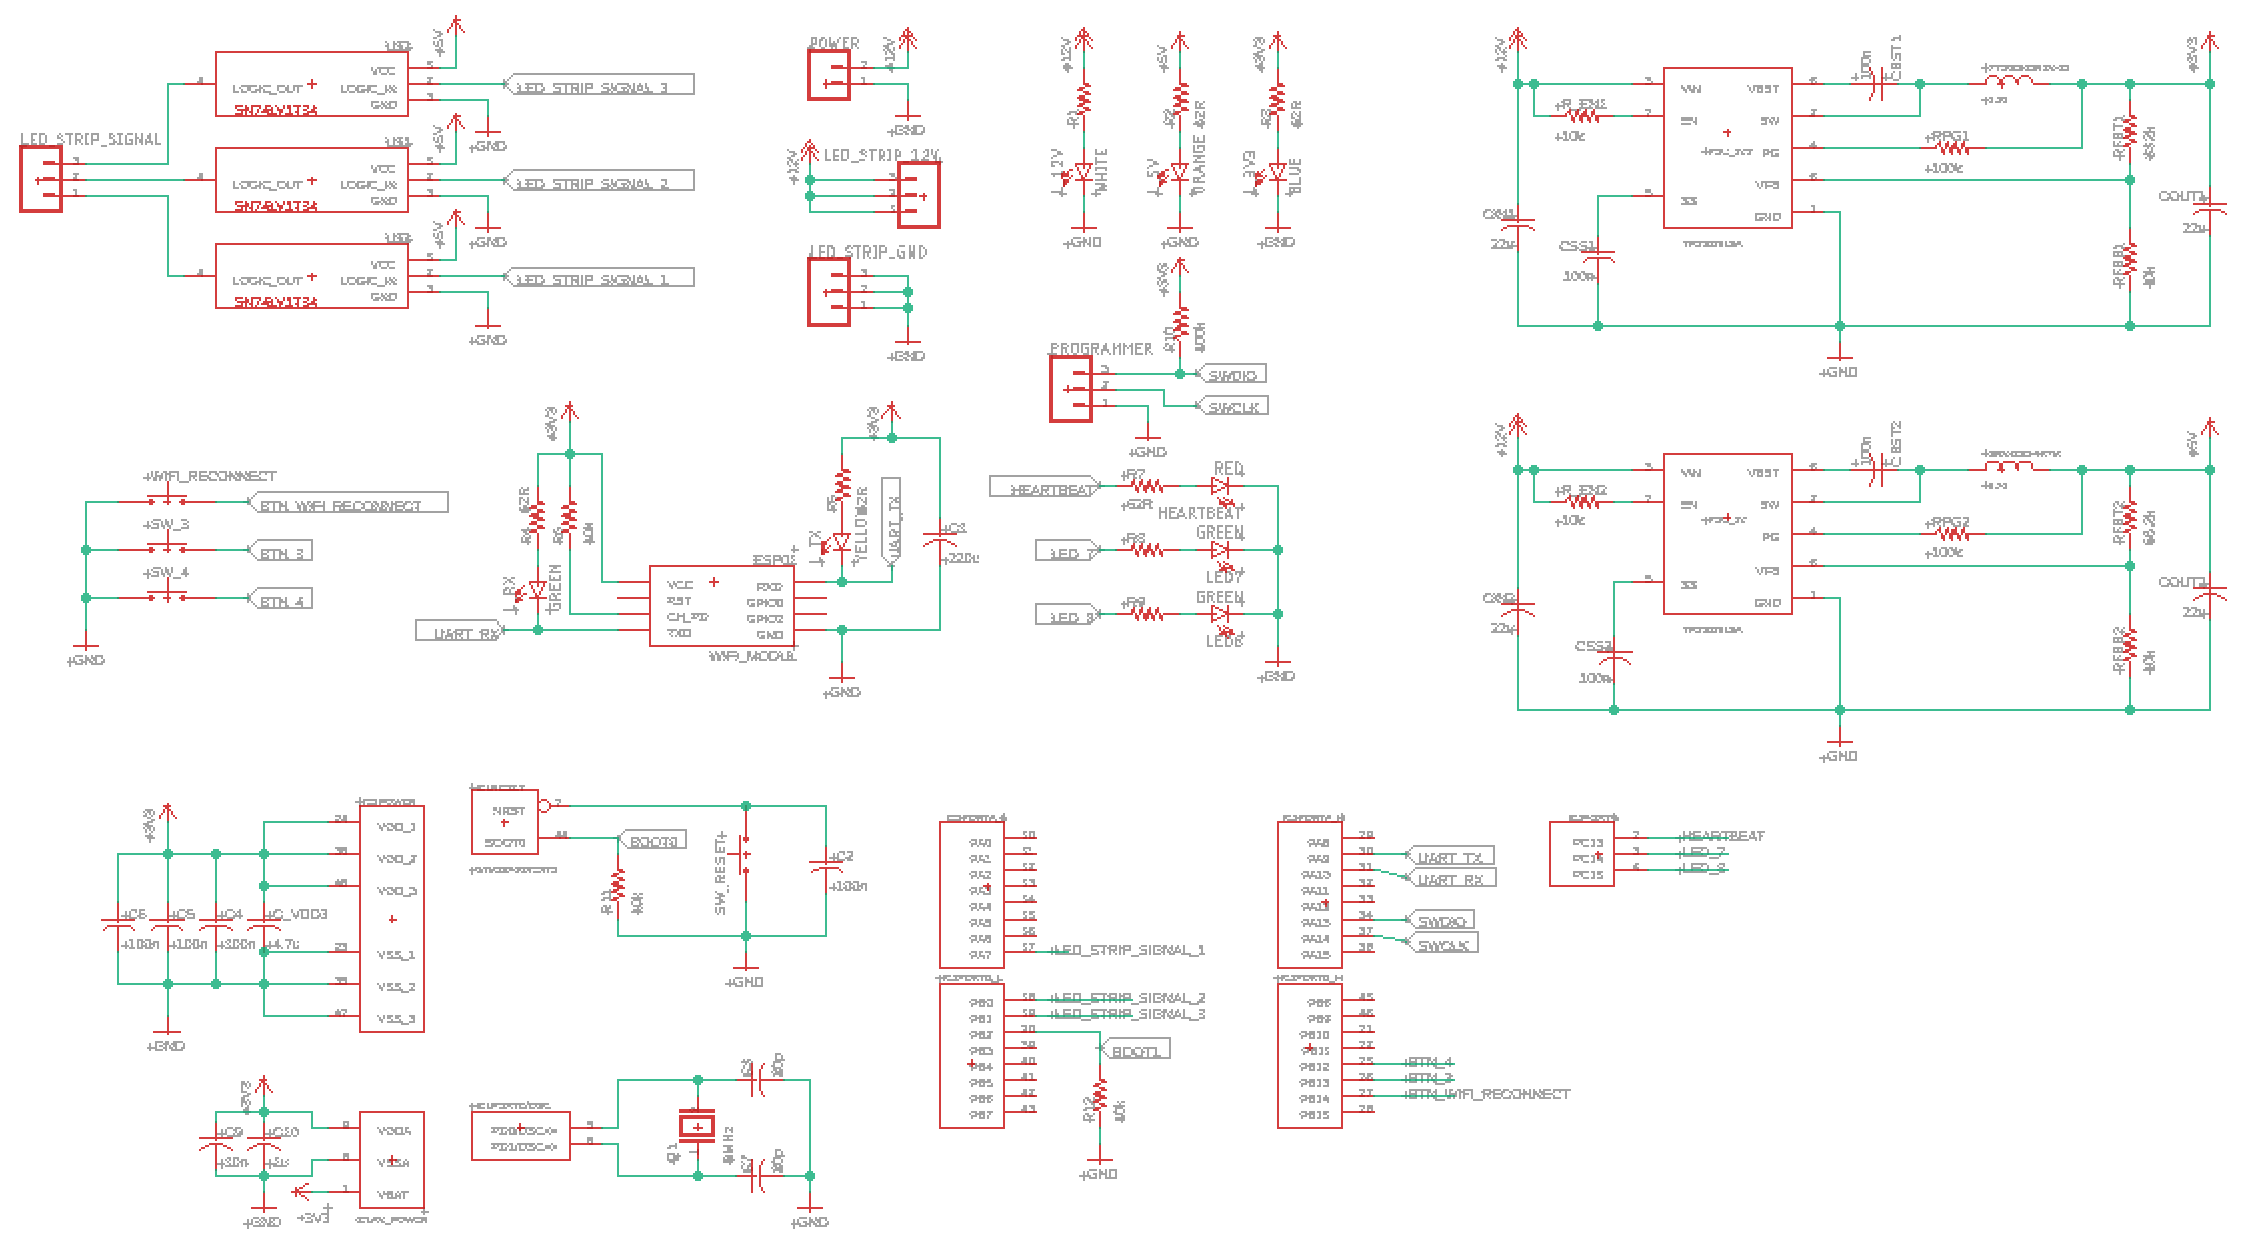
\includegraphics[width=12cm]{resources/pcb_res/schematic_v02.png}
                \caption{Lekicsinyített kapcsolási rajz (felnagyított verzió a függelékben található)}
                \label{fig:schamtic_v02}
            \end{figure}
            
            
            A kapcsolási rajz után az alkatrészek elhelyezése és huzalozása következett. Az EAGLE fejlesztői itt is nagy segítségemre voltak, és a 10 leghasznosabb tippet(//TODO ref) 
            % https://www.autodesk.com/products/eagle/blog/top-10-pcb-routing-tips-beginners/
            összegyűjtötték a témában nem annyira jártasak számára.
            A NYÁK-on logikai szempontok alapján elhelyeztem az alkatrészeket. A tápfeszültség és egyéb visszajelző LED-eket, gombokat - csoportonként - egymás mellé és a reset gombot a többi gombtól elkülönített helyre raktam. A LED sor és a Wifi modul kommunikációs jelvezetékeit minél távolabbra helyeztem a zajforrásoktól, mint például a DC/DC áramköröktől és az oszcillátor áramkörtől. Az elrendezett komponenseket összehuzaloztam a tervezési irányelvek és a fejlesztői tippek alapján (\ref{fig:board_v02}. ábra). 
            
            \begin{figure}[h!]
                \centering
                    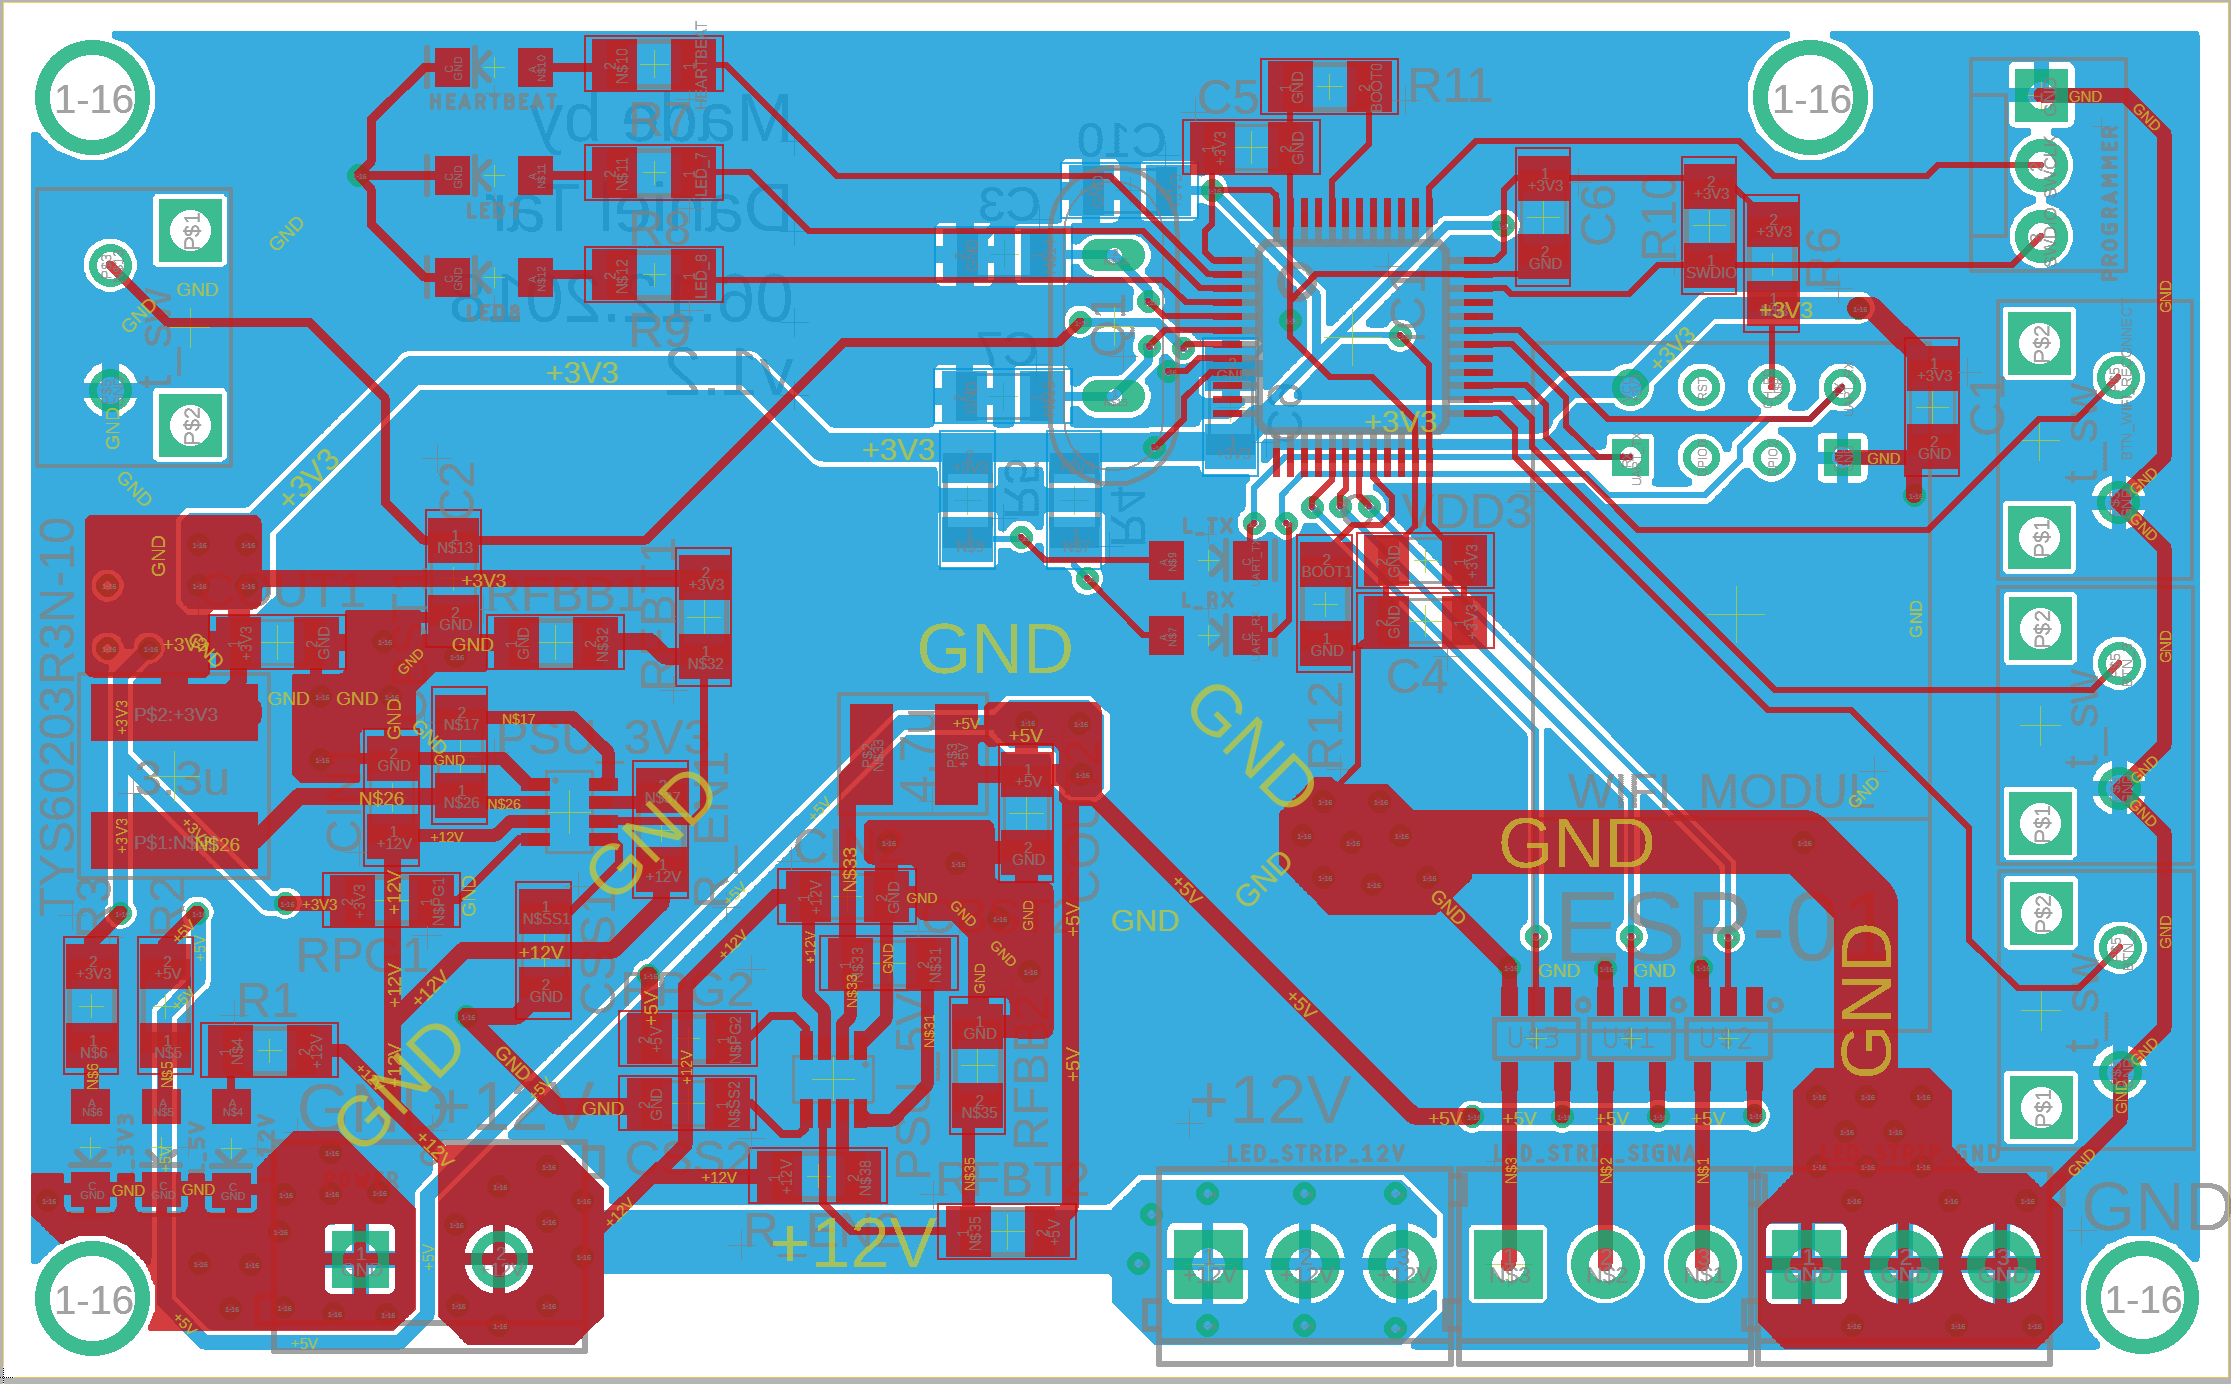
\includegraphics[width=12cm]{resources/pcb_res/board_v02.png}
                \caption{Összehuzalozott NYÁK terv}
                \label{fig:board_v02}
            \end{figure}
            
        \subsubsection{Alkatrészek megrendelése és a NYÁK legyártatása}
            
            Az alkatrészeimet az egyik legnagyobb internetes elektronikai viszonteladónál, a Mouser Electronics-nál, választatottam ki. A terveket úgy hoztam létre, hogy 1206-os mértetű alkatrészeket használtam, mert ezt a méretet nagy biztonsággal képes leszek beforrasztanni. A projekt nagy tanulsága viszont, hogy ebben a méretben egyátalán nem biztos, hogy minden értékben megtalálhatóak az alkatrészek, és ha igen, akkor is jellemzően jóval drágábban mint más méretekben. További probléma volt, hogy a TI Workbench által javasolt alkatrészek a DC/DC átalakítóhoz, kifutott termék révén, már elfogytak vagy nem is forgalmazták őket. A megfelelő szempontokra figyelve kiválasztottam az új alkatrészeket, frissítettem a kapcsolási rajzot és a NYÁK tervet (a frissített verzió képei találhatók az előző alfejezetben). 
            
            A sok NYÁK gyártó közül én a JLCPCB-t, egy prototípusgyártásra specializálódott céget, választottam. Az EAGLE-ben kigenerált gerber fáljokat (\ref{fig:gerber_v10}. ábra) kellett feltöltenem valamilyen tömörített állományként vagy zip vagy rar formátumban. Az alap beállításokat használva mindössze 2\$-ért + szállítási költségért két héten belül megkaptam.
            
            \begin{figure}[h!]
                \centering
                    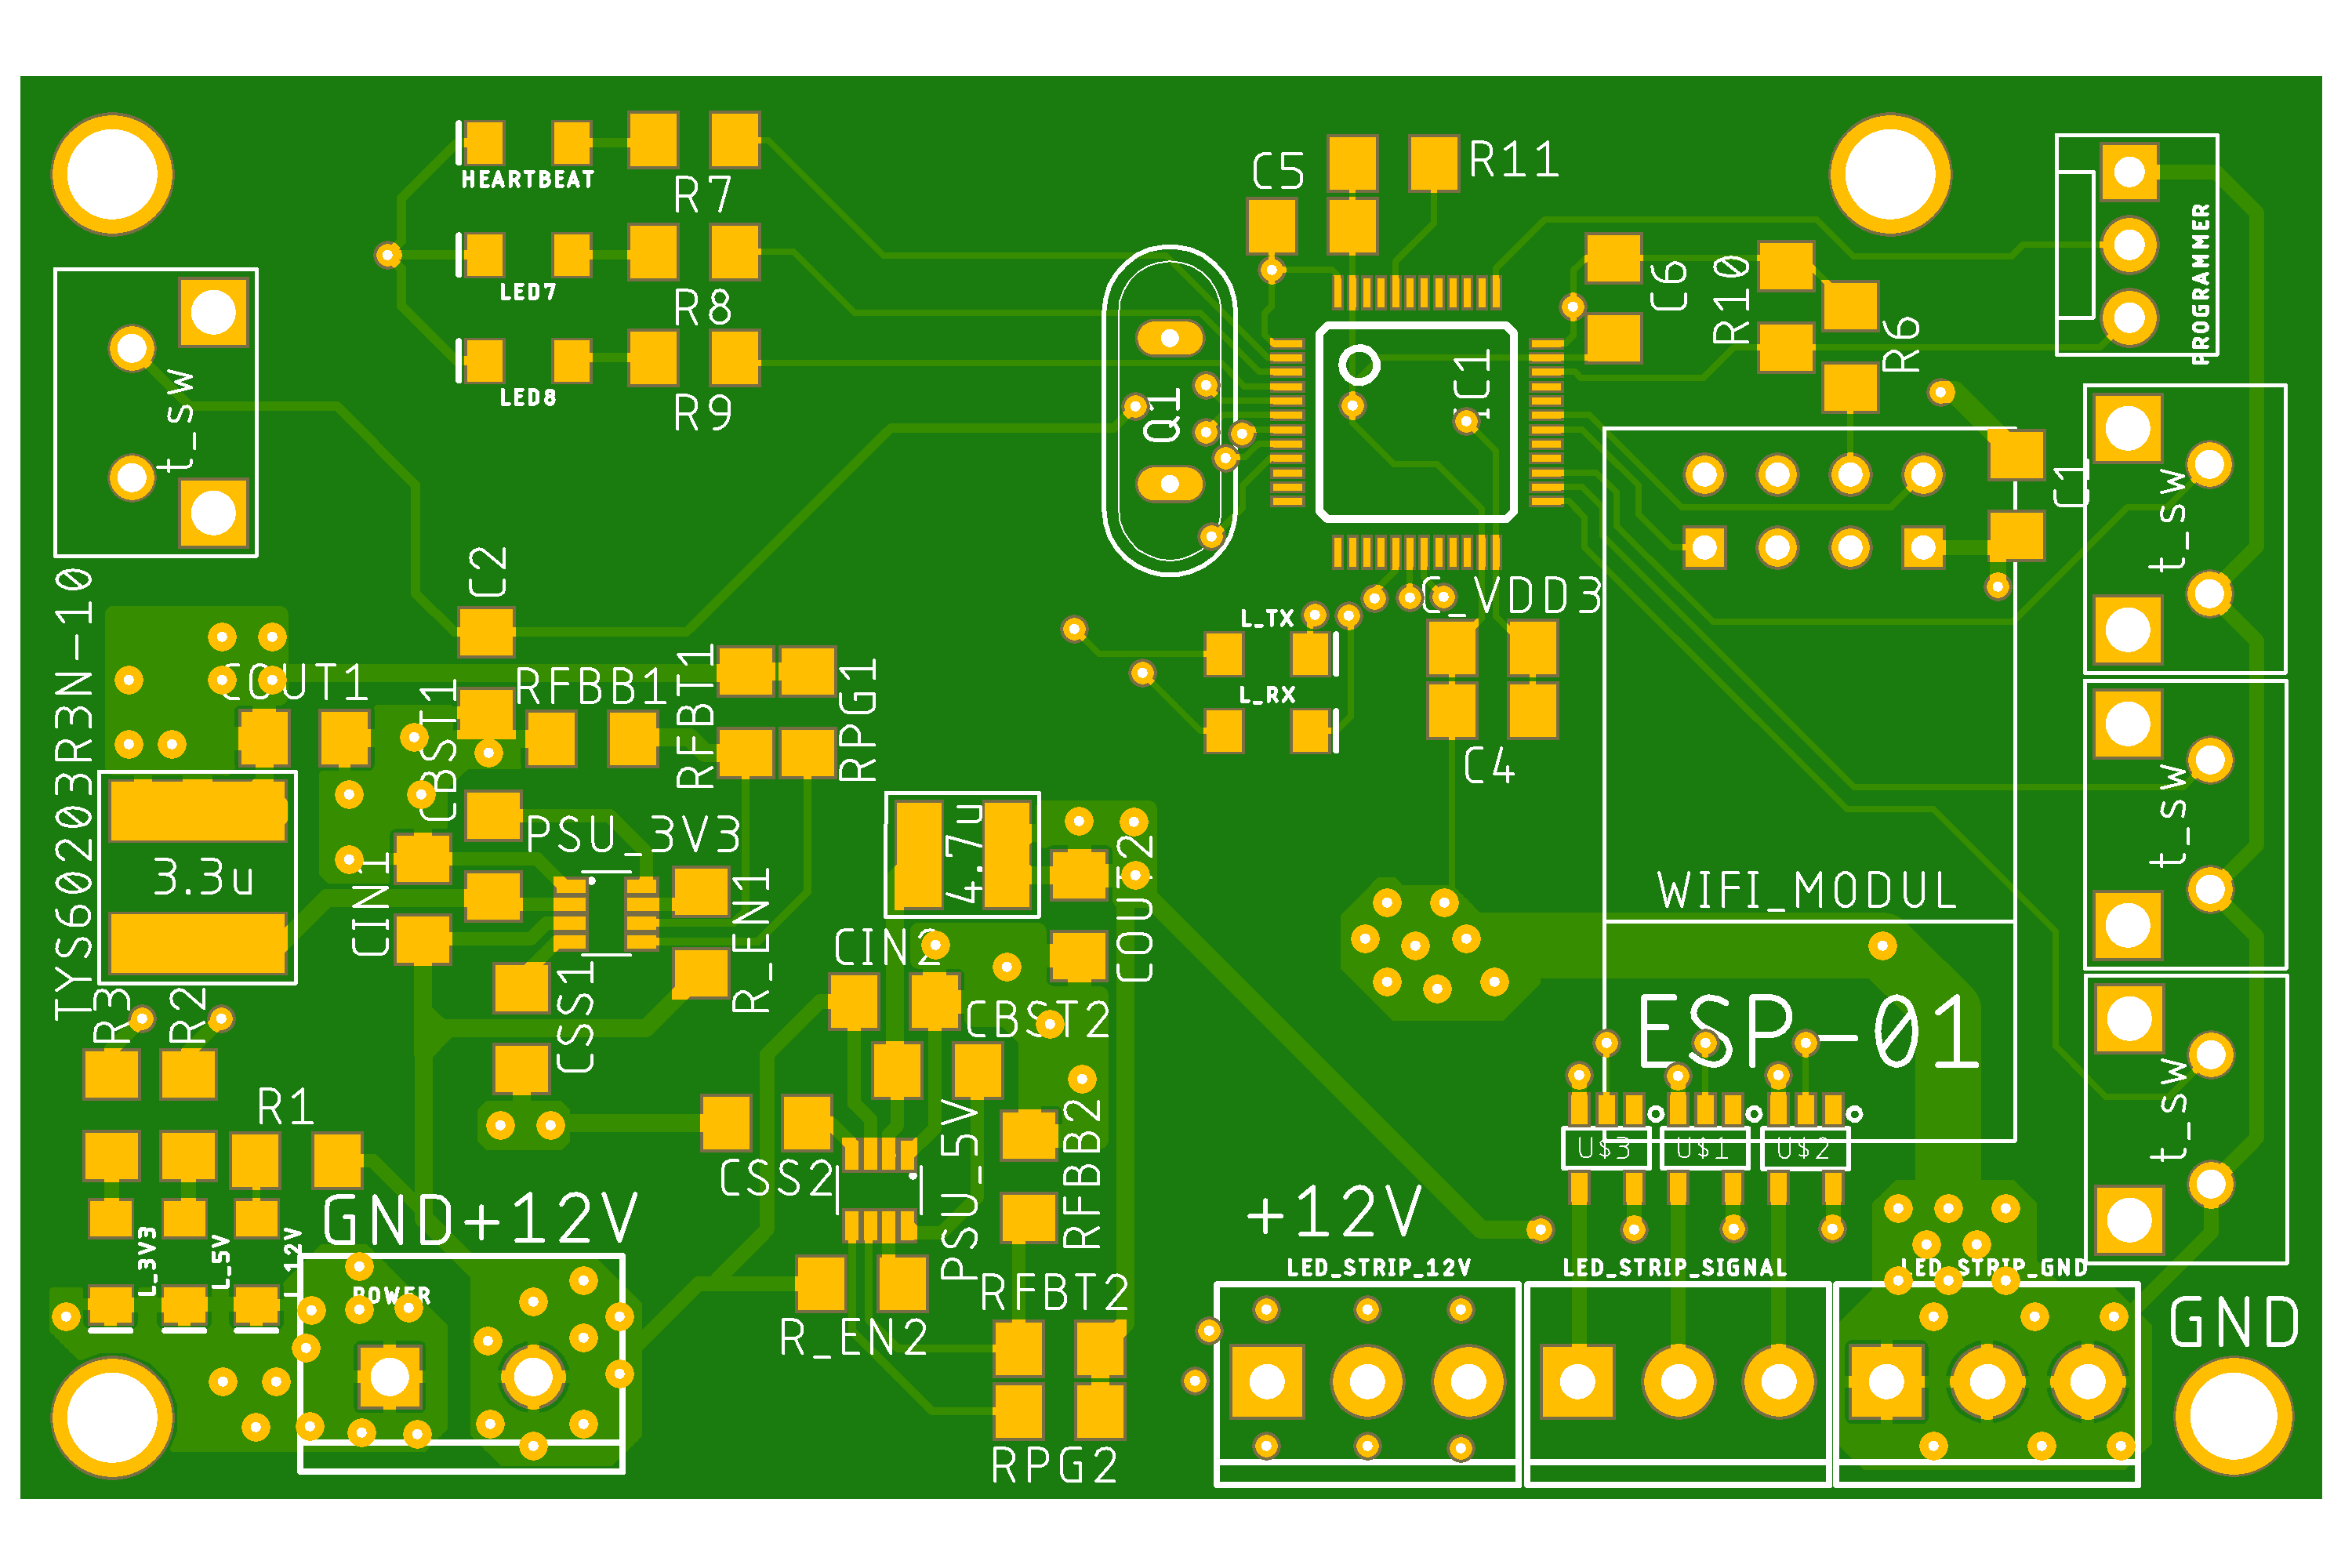
\includegraphics[width=7cm]{resources/pcb_res/pcb_top_v10.png}
                    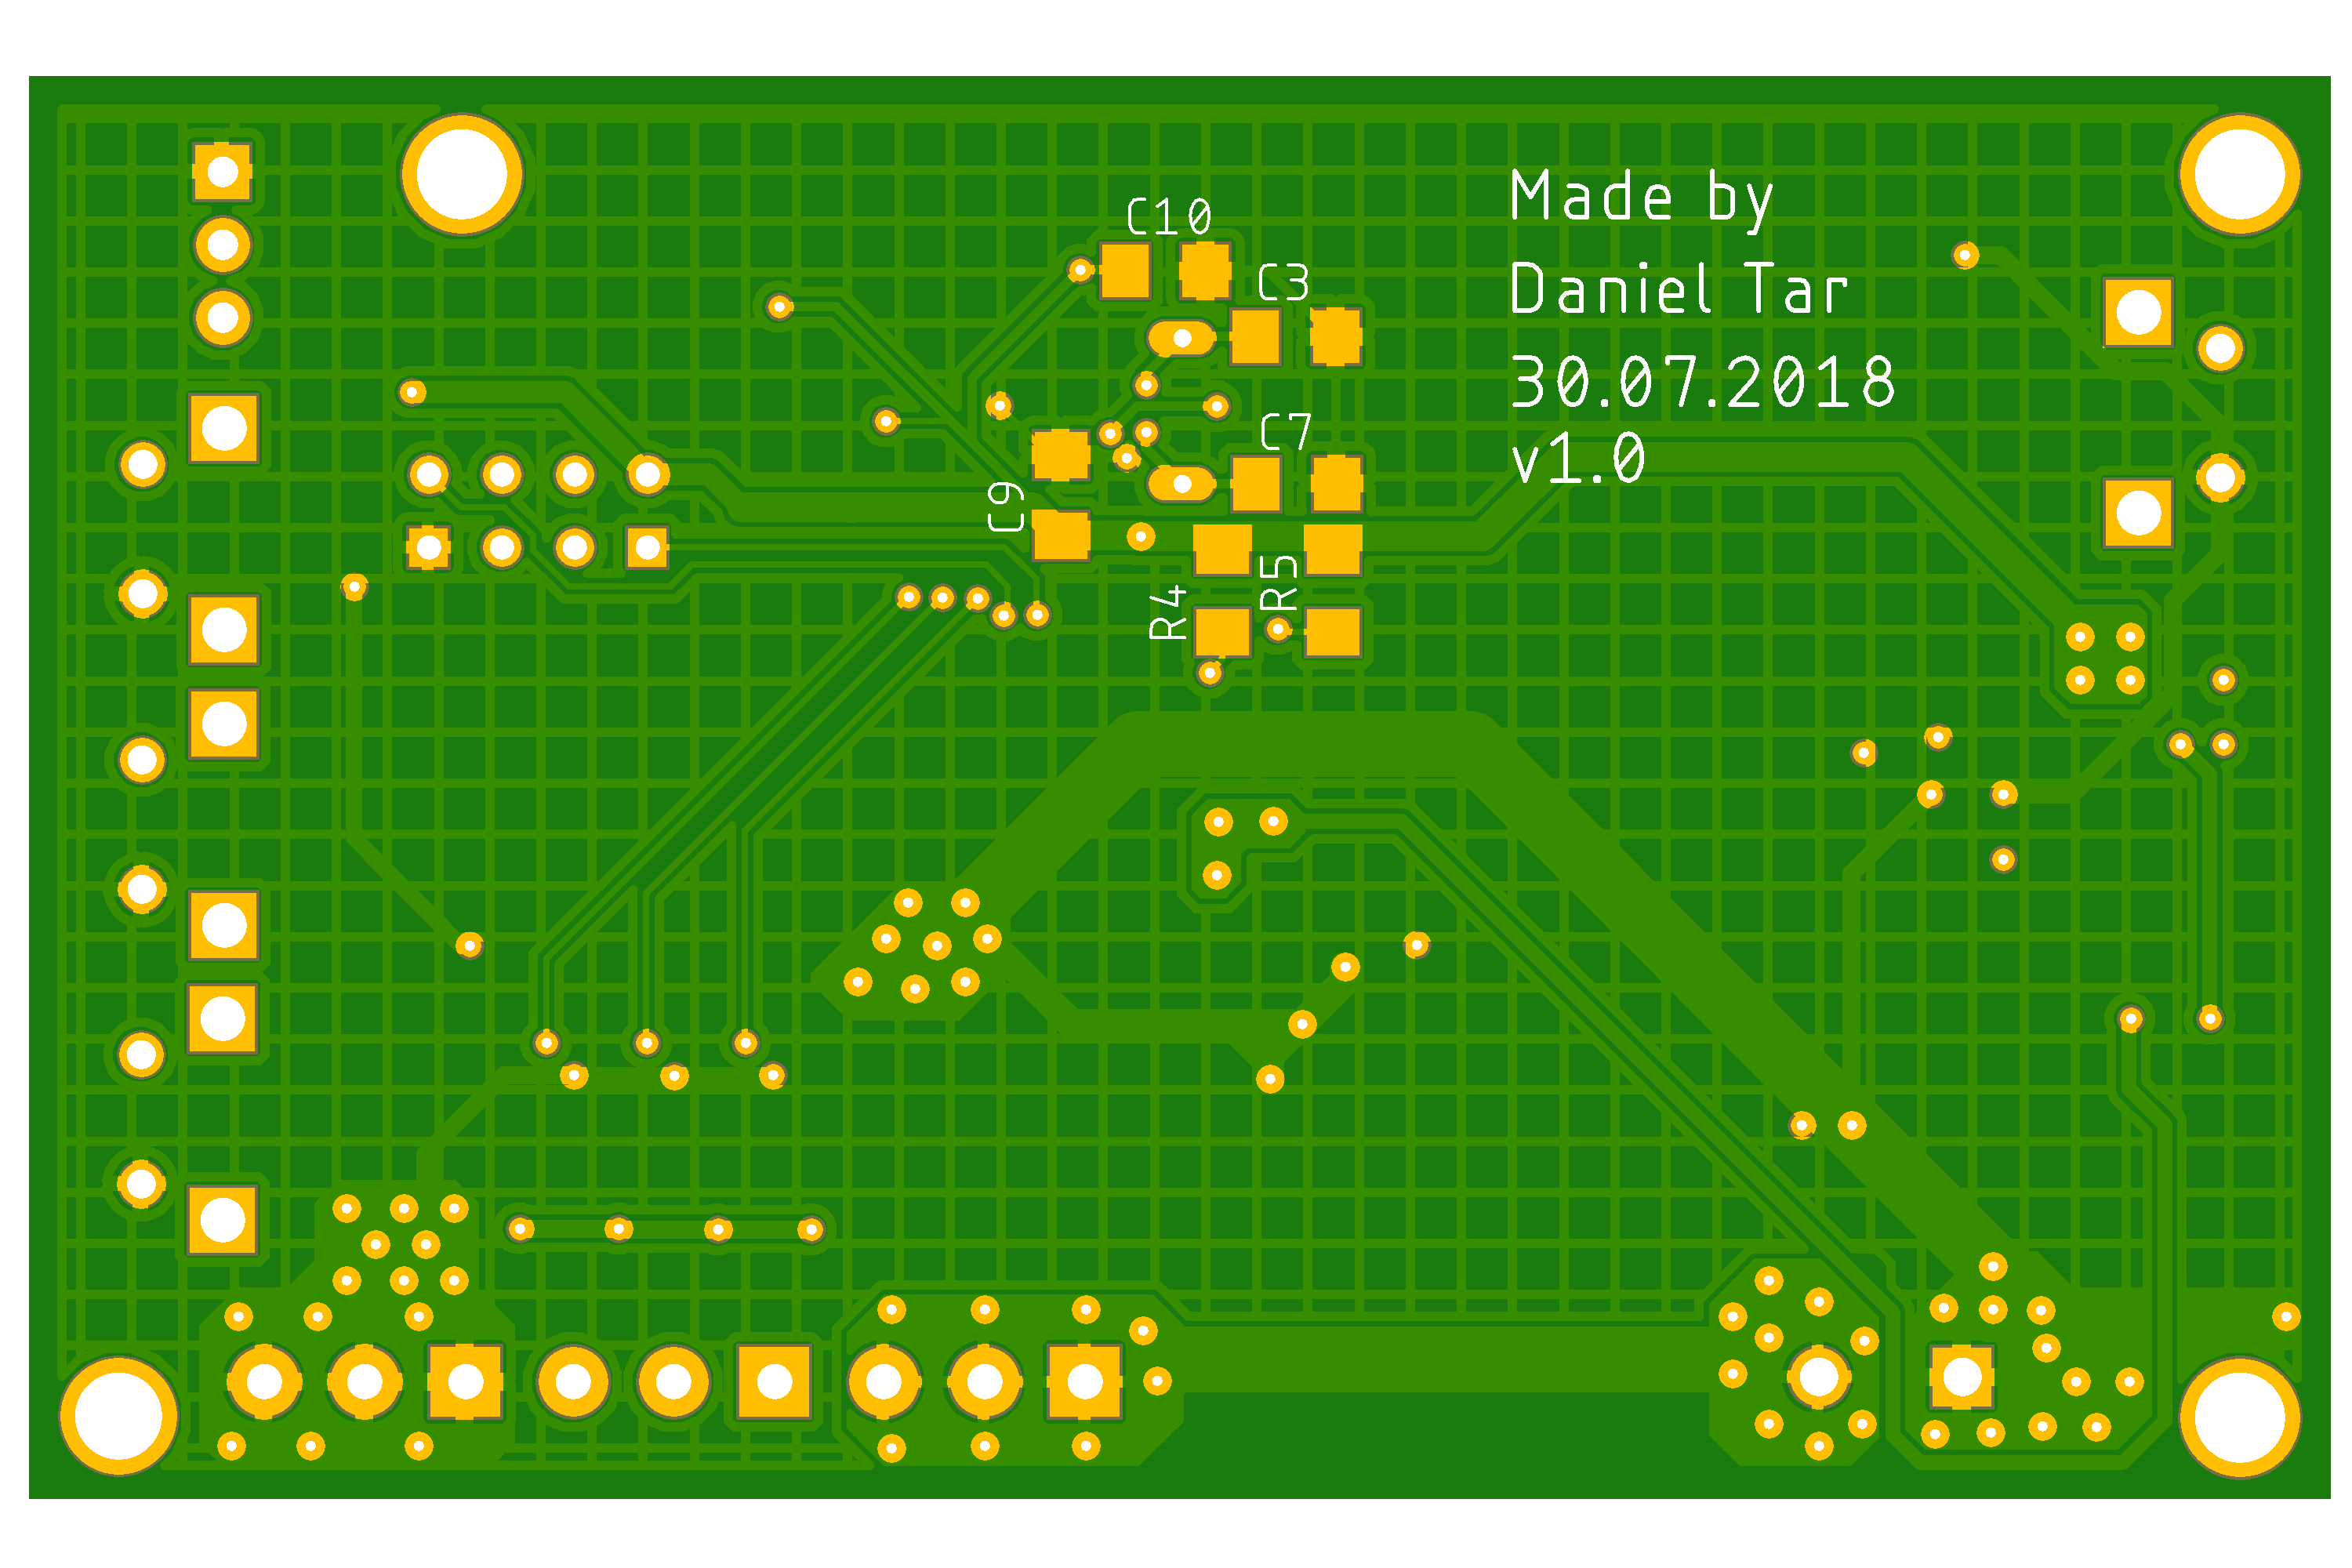
\includegraphics[width=7cm]{resources/pcb_res/pcb_bottom_v10.png}
                \caption{Gerber fájlok előnézetei}
                \label{fig:gerber_v10}
            \end{figure}

    \subsection{Az elkészült eszköz beforrasztása, tesztelése}
        Az eszközt fokozatosan készítettem el, rész egységenként haladva. Először beforrasztottam, majd ellenőriztem a csatlakozásokat, rövidrezárást multiméterrel (diódateszter funkció). Ha nem sikerült valamit rendesen beforrasztani, akkor megpróbáltam még egyszer, és utána újra ellenőriztem a dolgok helyességét. Amennyiben mindent rendben találtam, akkor rákötöttem az eszközöm a labortápra (megfelelő feszültséget, és áramkorlátozást beállítva) és oszcilloszkóppal mértem a megfelelő működést. Szépen haladtam sorban a 3,3V-os, az 5V-os DC/DC, a mikrokontroller és a többi részen. Többnyire első, STM32F103-as IC-nél második próbálkozásra elkészült az első prototípus. 
        
        Jöhetett a szoftveres tesztelés. Az első és legfontossabb az volt, hogy programozható-e a mikrokontroller, vagy sem. 10 alkalomból 7-szer sikerült is felprogramozni az IC-t, ami nem éppen az elvárt működés volt. További tesztek során a Wifi modulall való kommunikációt is sikeresen leteszteltem. Az egyik bekapcsolásnál viszont váratlanul kisült az egyik táp IC. Huzamosabb kísérletezés után, megismétlődött az előbbi eset és elkezdtem keresni a probléma okát. Időbe telt, mire kiderült, hogy a táp IC EAGLE könyvtárának készítése során felcseréltem két lábat. Viszont a hiba kijavítása után sem szűnt meg az eredeti probléma. A végső megoldást az úgynevezett \textit{Soft Start} kondenzátor (C$_{SS}$) kicserélése jelentette. Ez a kondenzátor felelős azért, hogy milyen gyorsan kapcsoljon be, és állítsa be a kimeneti feszültséget a DC/DC áramkör. A TI Workbench által javasolt 8,2nF értéket 100nF-ra cseréltem, amivel a készülék azóta is jól működik. Ezzel az értékkel 20ms felfutási ideje lett a tápfeszültségeknek.
        
        \begin{figure}[h!]
            \centering
                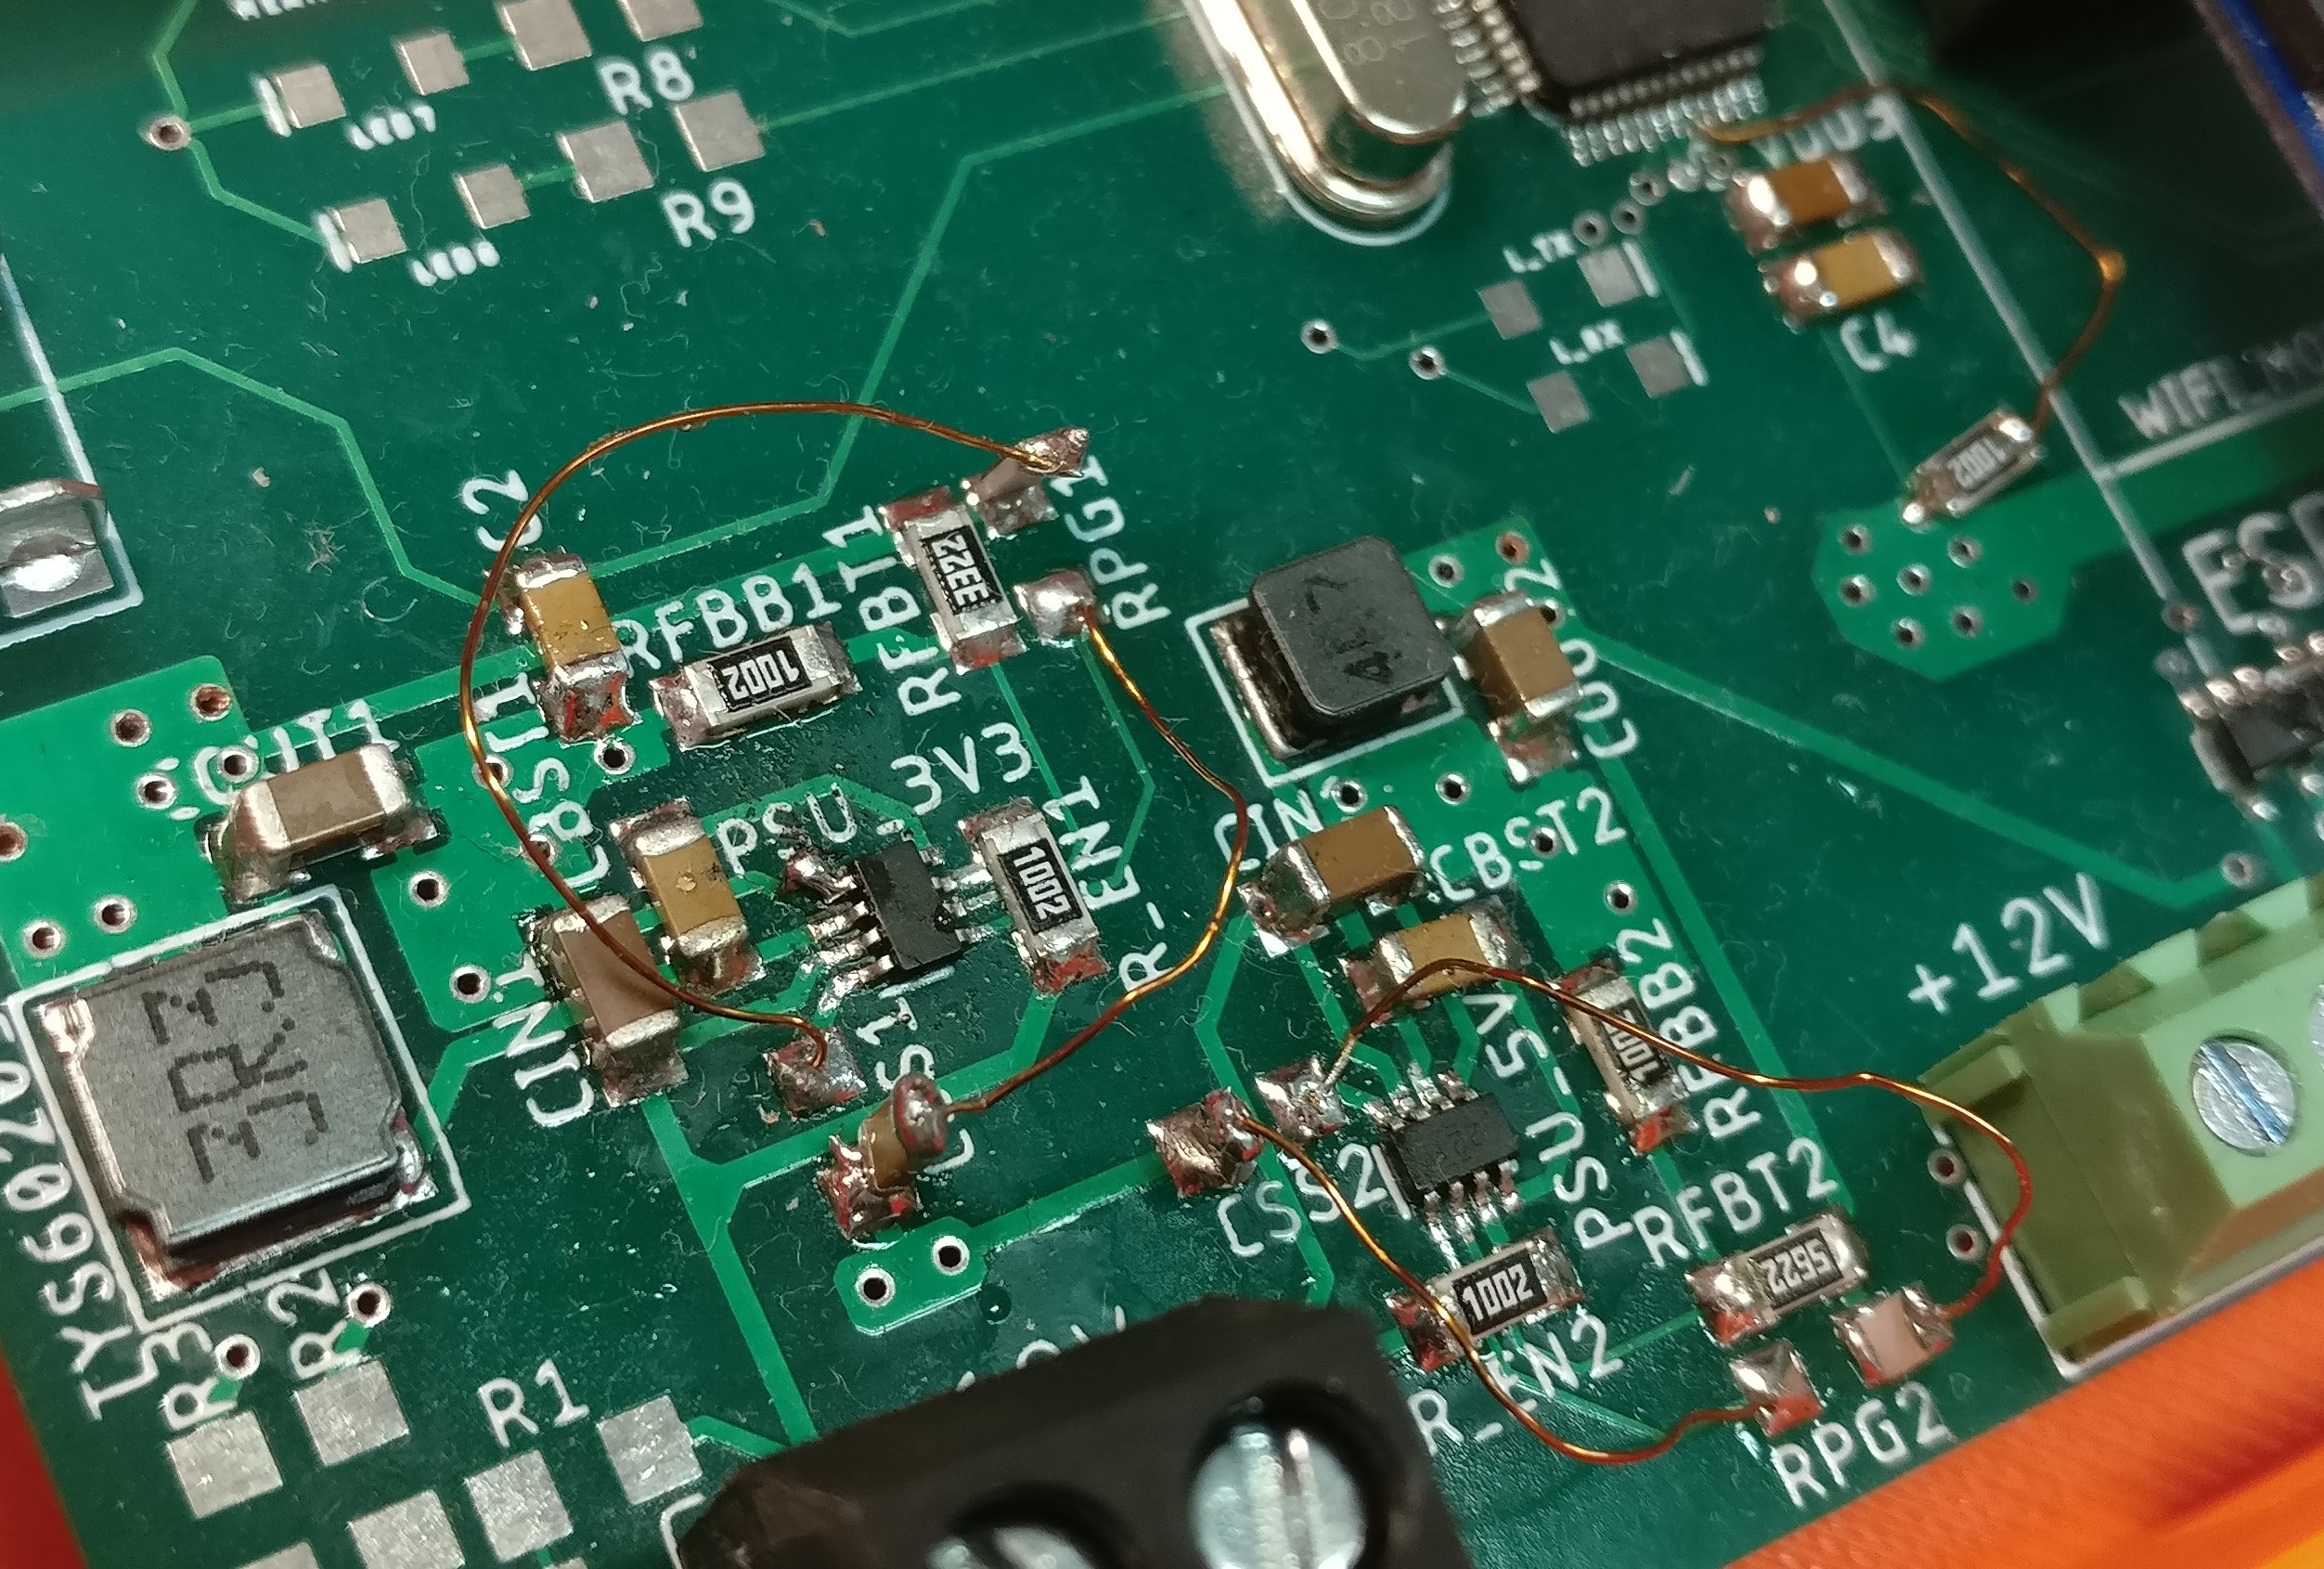
\includegraphics[width=8cm]{resources/pcb_res/pcb_psu_lib_fail}
            \caption{A táp IC felcserélt lábainak kijavítása az elkészült NYÁK-on}
            \label{fig:pcb_psu_fail}
        \end{figure}
        
        Az eszköznek jelenleg hálós föld rétege van, mert az első verzió tervezésénél úgy emlékeztem, hogy ennek előnyösebb tulajdonságai vannak mint az egybefüggő földrétegnek. Azóta utána jártam (TODO \ref{}), és kiderült, hogy az egybefüggő sokszor jobb. A NYÁK terven ez kijavításra került, de azóta még nem került legyártásra.
        %https://electronics.stackexchange.com/questions/5139/solid-ground-plane-vs-hatched-ground-plane
        
    \subsection{Védődoboz tervezése, 3D-nyomtatással prototípus gyártása}
    
        \subsubsection{Védődoboz 3D modellezése}
            Az utóbbi időben egyre gyosabban fejlődik az EAGLE. Megjelentek a 3D-s alkatrészkönyvtárak, és az Autodesk Fusion 360 (továbbiakban Fusion) nevű programba való exportálás, feltöltés lehetősége is. A Fusion egy felhő alapú program CAD, CAM és CAE eszközökkel. A felhő alapú szolgáltatás lényege, hogyha a NYÁK tervet az EAGLE-ben frissítem, akkor az Autodesk szerverein is frissül, ezáltal a Fusion-be érzékelve a változtatásokat.
            A NYÁK-ot és a grabcad.com oldalról letöltött Wifi modult beimportáltam és összeillesztettem (\ref{fig:fusion_pcb_esp8266}. ábra).
            
            \begin{figure}[h!]
                    \centering
                        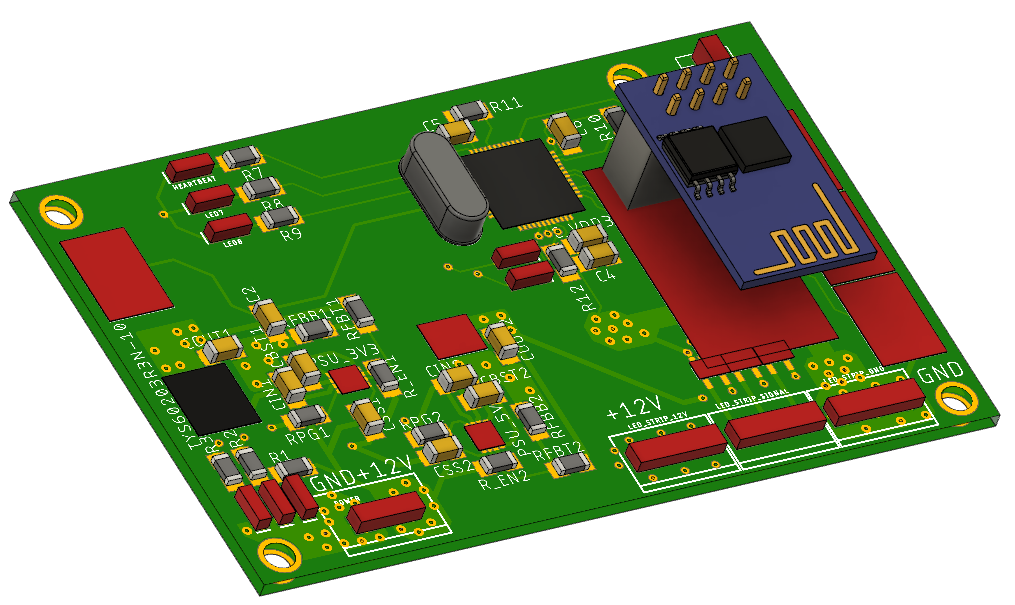
\includegraphics[width=8cm]{resources/pcb_res/fusion_pcb_esp8266.png}
                    \caption{Fusion-be importált NYÁK és ESP8266-os Wifi modul}
                    \label{fig:fusion_pcb_esp8266}
            \end{figure}
            
            Az elektronikai részek 3D-s környezetbe illesztése után elkezdtem a védődoboz modellezését. Parametrikus modellezést és a NYÁK referenciaméreteit használtam a gyors testreszabhatóság és az automatikus méretváltozás miatt. A dobzon nyílást hagytam a tápvezetékek, LED sorok bekötésére, a programozó csatlakozónak. Furatot készítettem a reset gomb számára, hogy szükség esetén benyomható legyen, illetve a 3 a házon elhelyezett nyomógombot kapott a 3 extra kapcsoló.
            
            //ábra a változtatható paraméterekről kell/nem?
            % \begin{figure}[h!]
            %     \centering
            %         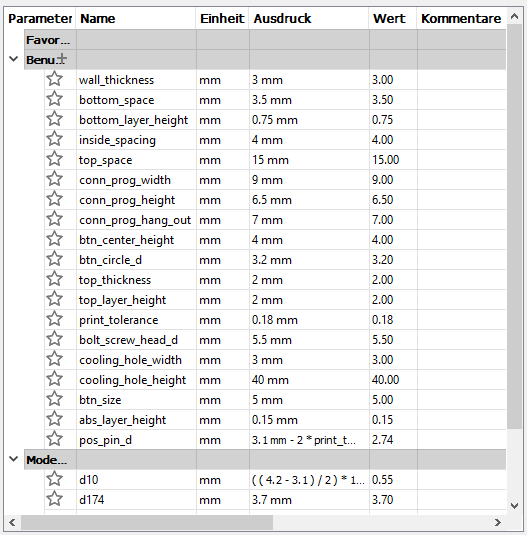
\includegraphics[height=5.5cm]{resources/pcb_res/fusion_parameter_list.png}
            %         \caption{Változtatható paraméterek}
            %         \label{fig:fusion_parameters}
            % \end{figure}
            
            \begin{figure}[h!]
                \centering
                    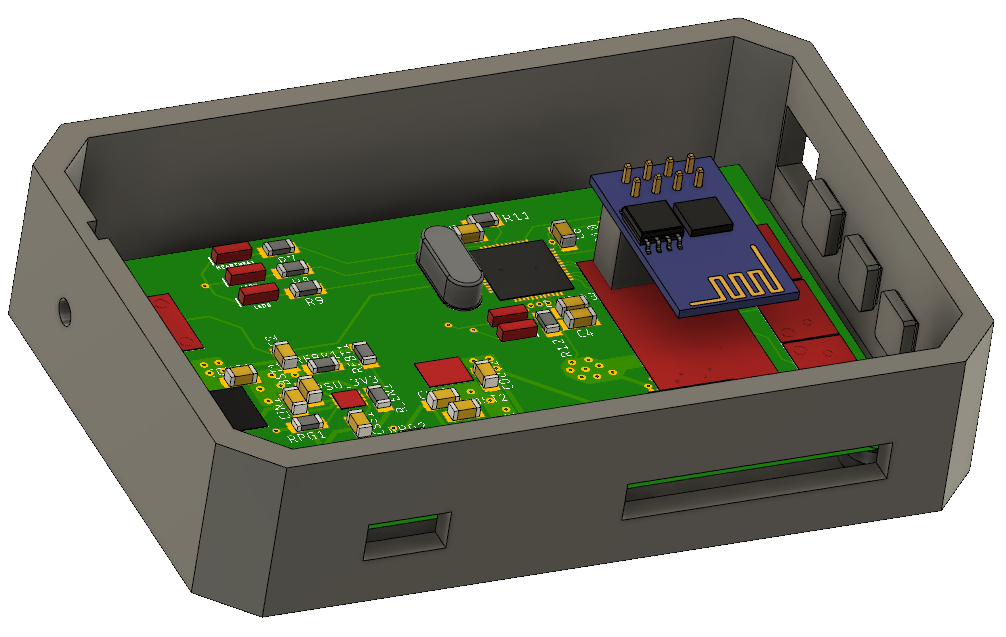
\includegraphics[width=7.5cm]{resources/pcb_res/fusion_case_body.png}
                    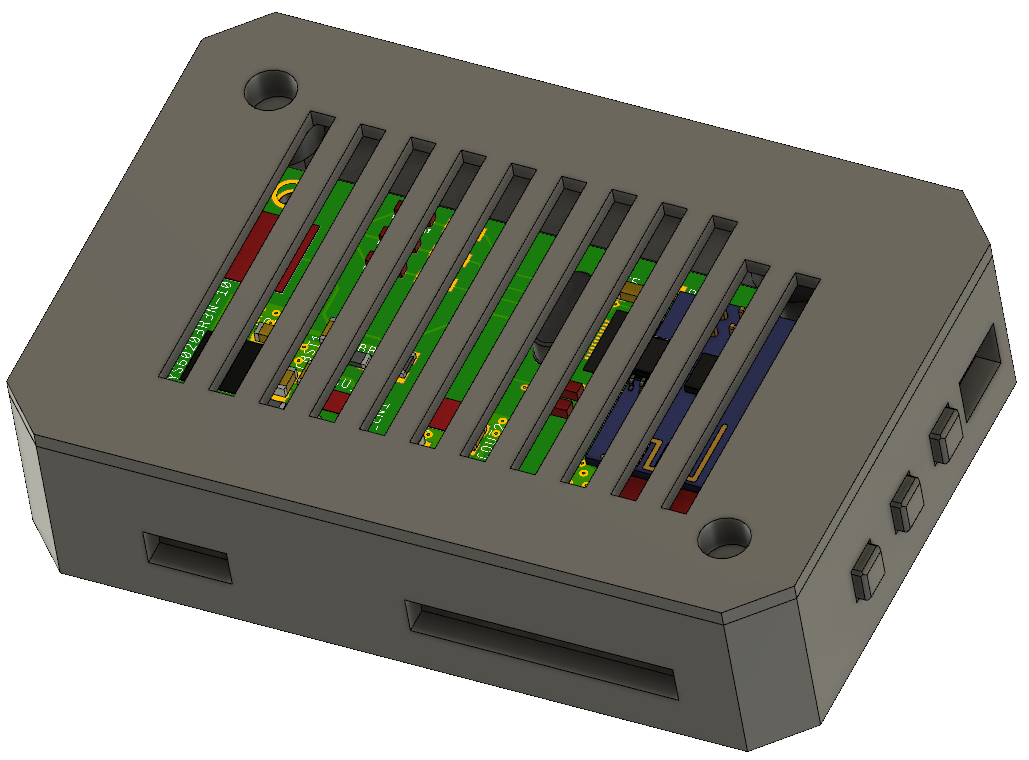
\includegraphics[width=7.5cm]{resources/pcb_res/fusion_case_cooling_ribs.png}
                    % 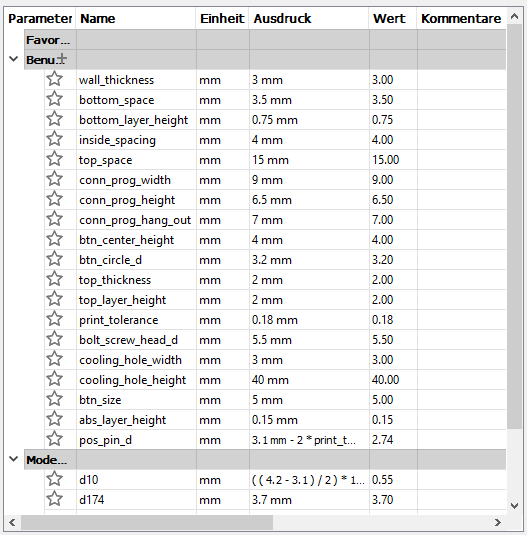
\includegraphics[width=7.5cm]{resources/pcb_res/fusion_parameter_list.png}
                    \caption{Védődoboz 3D-s tervei}
                    \label{fig:fusion_case_body}
            \end{figure}
            
            \begin{figure}[h!]
                \centering
                    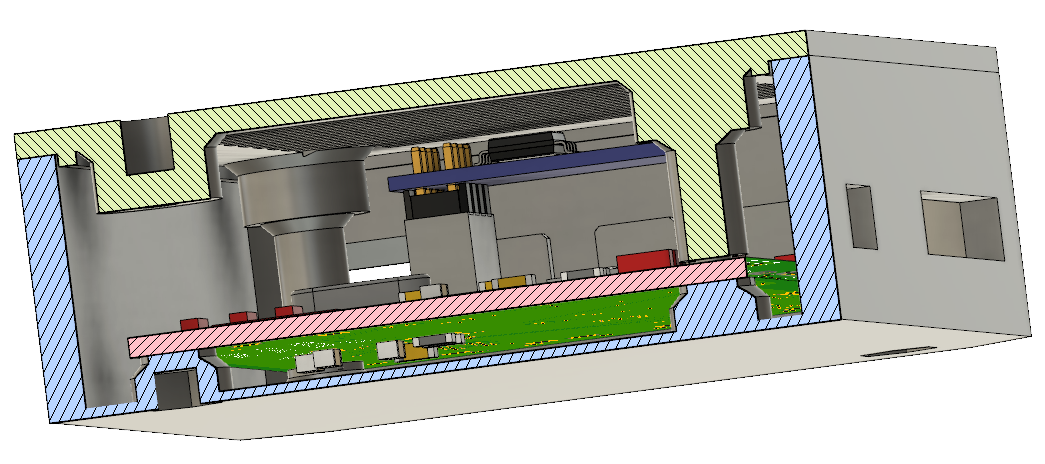
\includegraphics[width=7.5cm]{resources/pcb_res/fusion_case_cut.png}
                    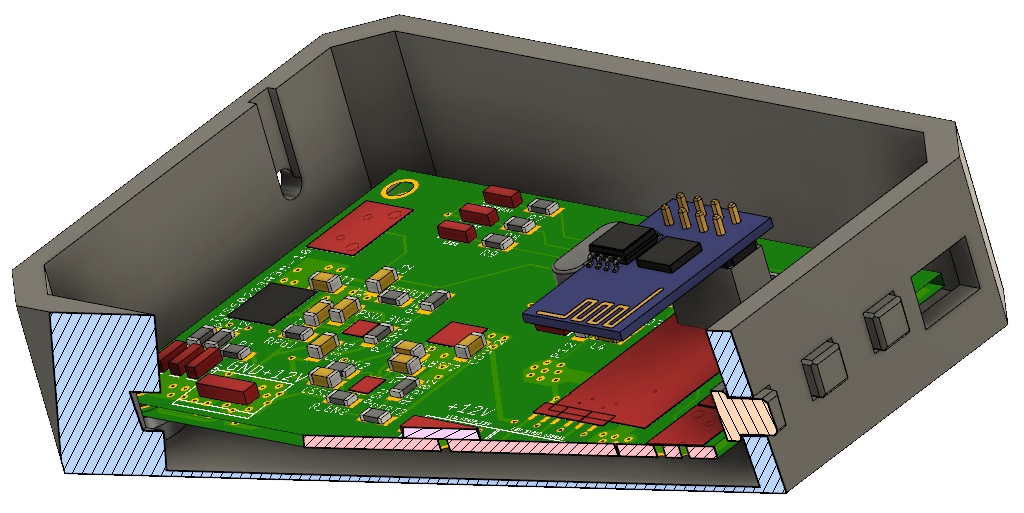
\includegraphics[width=7.5cm]{resources/pcb_res/fusion_case_cut2.png}
                    \caption{3D-s tervek metszetben}
                    \label{fig:fusion_case_body_cut}
            \end{figure}
            
            A NYÁK-on 4 furat található, ebből kettőt a dobozban való pozícionálásra használtam, kettőt pedig a doboz házának és fedelének a rögzítésére. A fedélből több verziót is készítettem. Az egyiken hálós hűtő felület került elhelyezésre és főleg benti használatra lett tervezve, míg a másik teljesen zárt testtel rendelkezik. Az otthoni terasz megvilágításra például a zárt verziójút szereltem fel az eresz alá. 
            
            % \begin{figure}[h!]
            %     \centering
            %         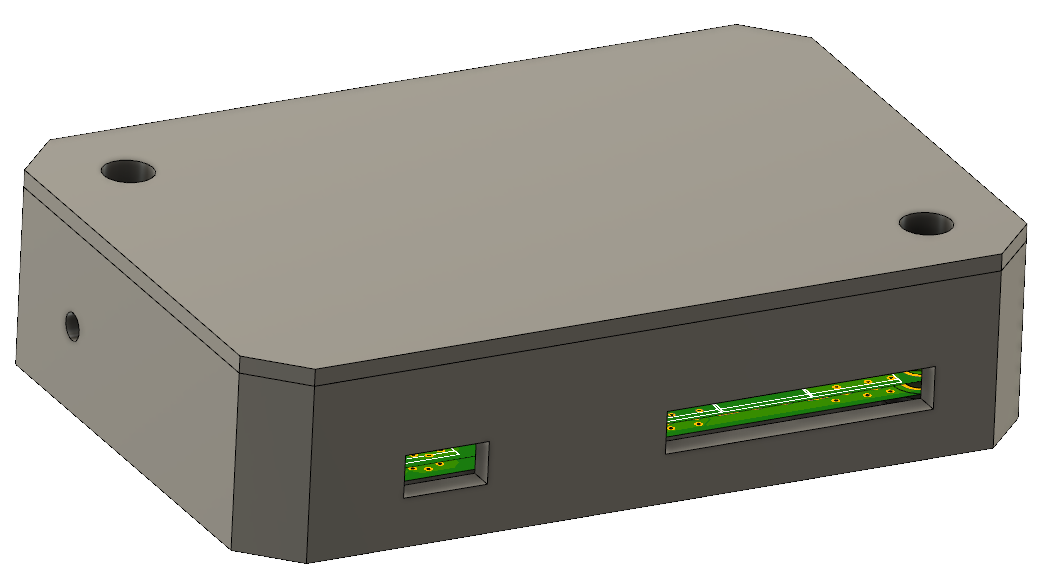
\includegraphics[width=7.5cm]{resources/pcb_res/fusion_case_closed.png}
            %         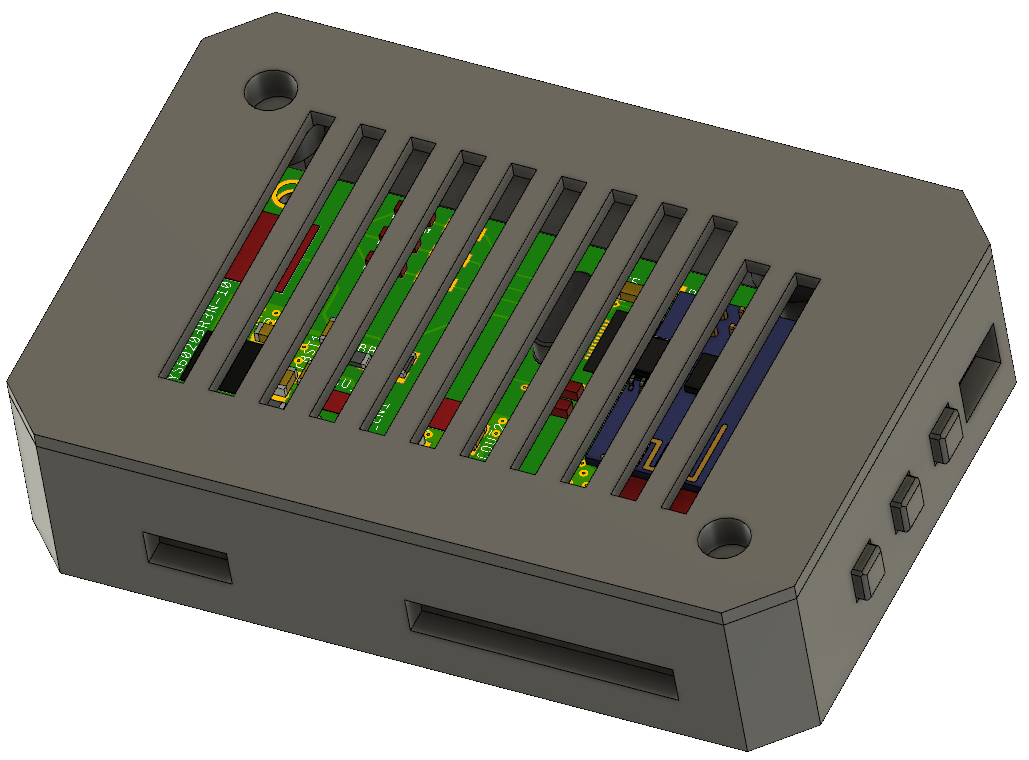
\includegraphics[width=7.5cm]{resources/pcb_res/fusion_case_cooling_ribs.png}
            %         \caption{Zárt és nyitott fedő}
            %         \label{fig:fusion_case_top}
            % \end{figure}
        
        \subsubsection{3D nyomtatás és az elkészült hardver}
            Manapság a 3D nyomtatás a prototípusgyártás megkerülhetetlen része lett. Olcsón, gyorsan, valós mértetű, mérethelyes alkatrészeket készíthetünk. A meglévő technológiák közül a számomra elérhető FDM-et (Fused Deposition Modelling) használtam. A módszer lényege, hogy egy megfelelő polimertekercsből, rétegenként állítjuk elő a kivánt modellünket. Slic3r PE egy olyan program, ami elvégzi a modellünk slice-olását (\ref{fig:ledstrip_case_slice}. ábra) (rétegekre bontását), és a 3D nyomtató számára legenerálja a megfelelő G-Code-ot. Ez a kód tartalmazza azokat az információkat, hogy milyen hőmérsékletre kell fűteni az adott anyagot, mikor, milyen sebességgel és hova kell mozogjon az extruder (nyomtató fej). 
            
            \begin{figure}[h!]
                \centering
                    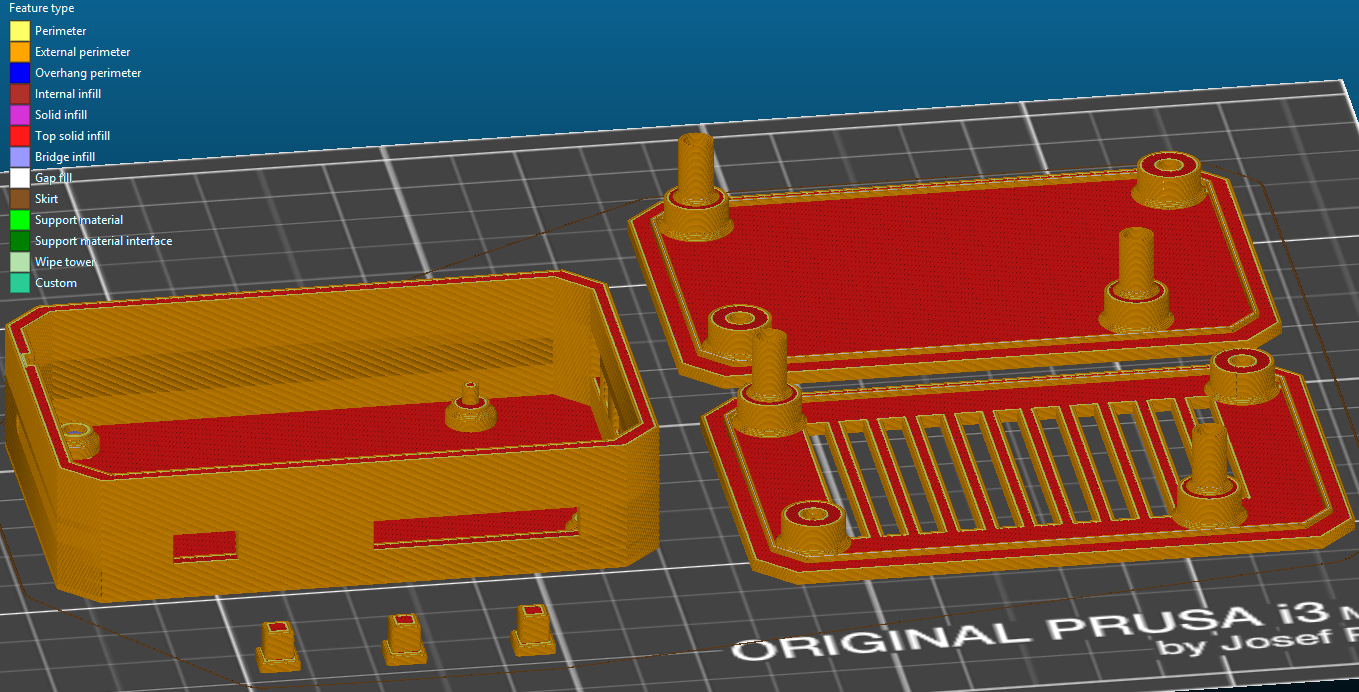
\includegraphics[width=13.5cm]{resources/pcb_res/slic3r_ledstrip_case.png}
                    \caption{Védődoboz slice-olás után}
                    \label{fig:ledstrip_case_slice}
            \end{figure} 
            
            A nyomtatás után összeszerelt és beforrasztott ledsorvezérlőket \aref{fig:printed_cases_1}. és \aref{fig:printed_cases_2}. Ábrák szemléltetik.
            
            \begin{figure}[h!]
                \centering
                    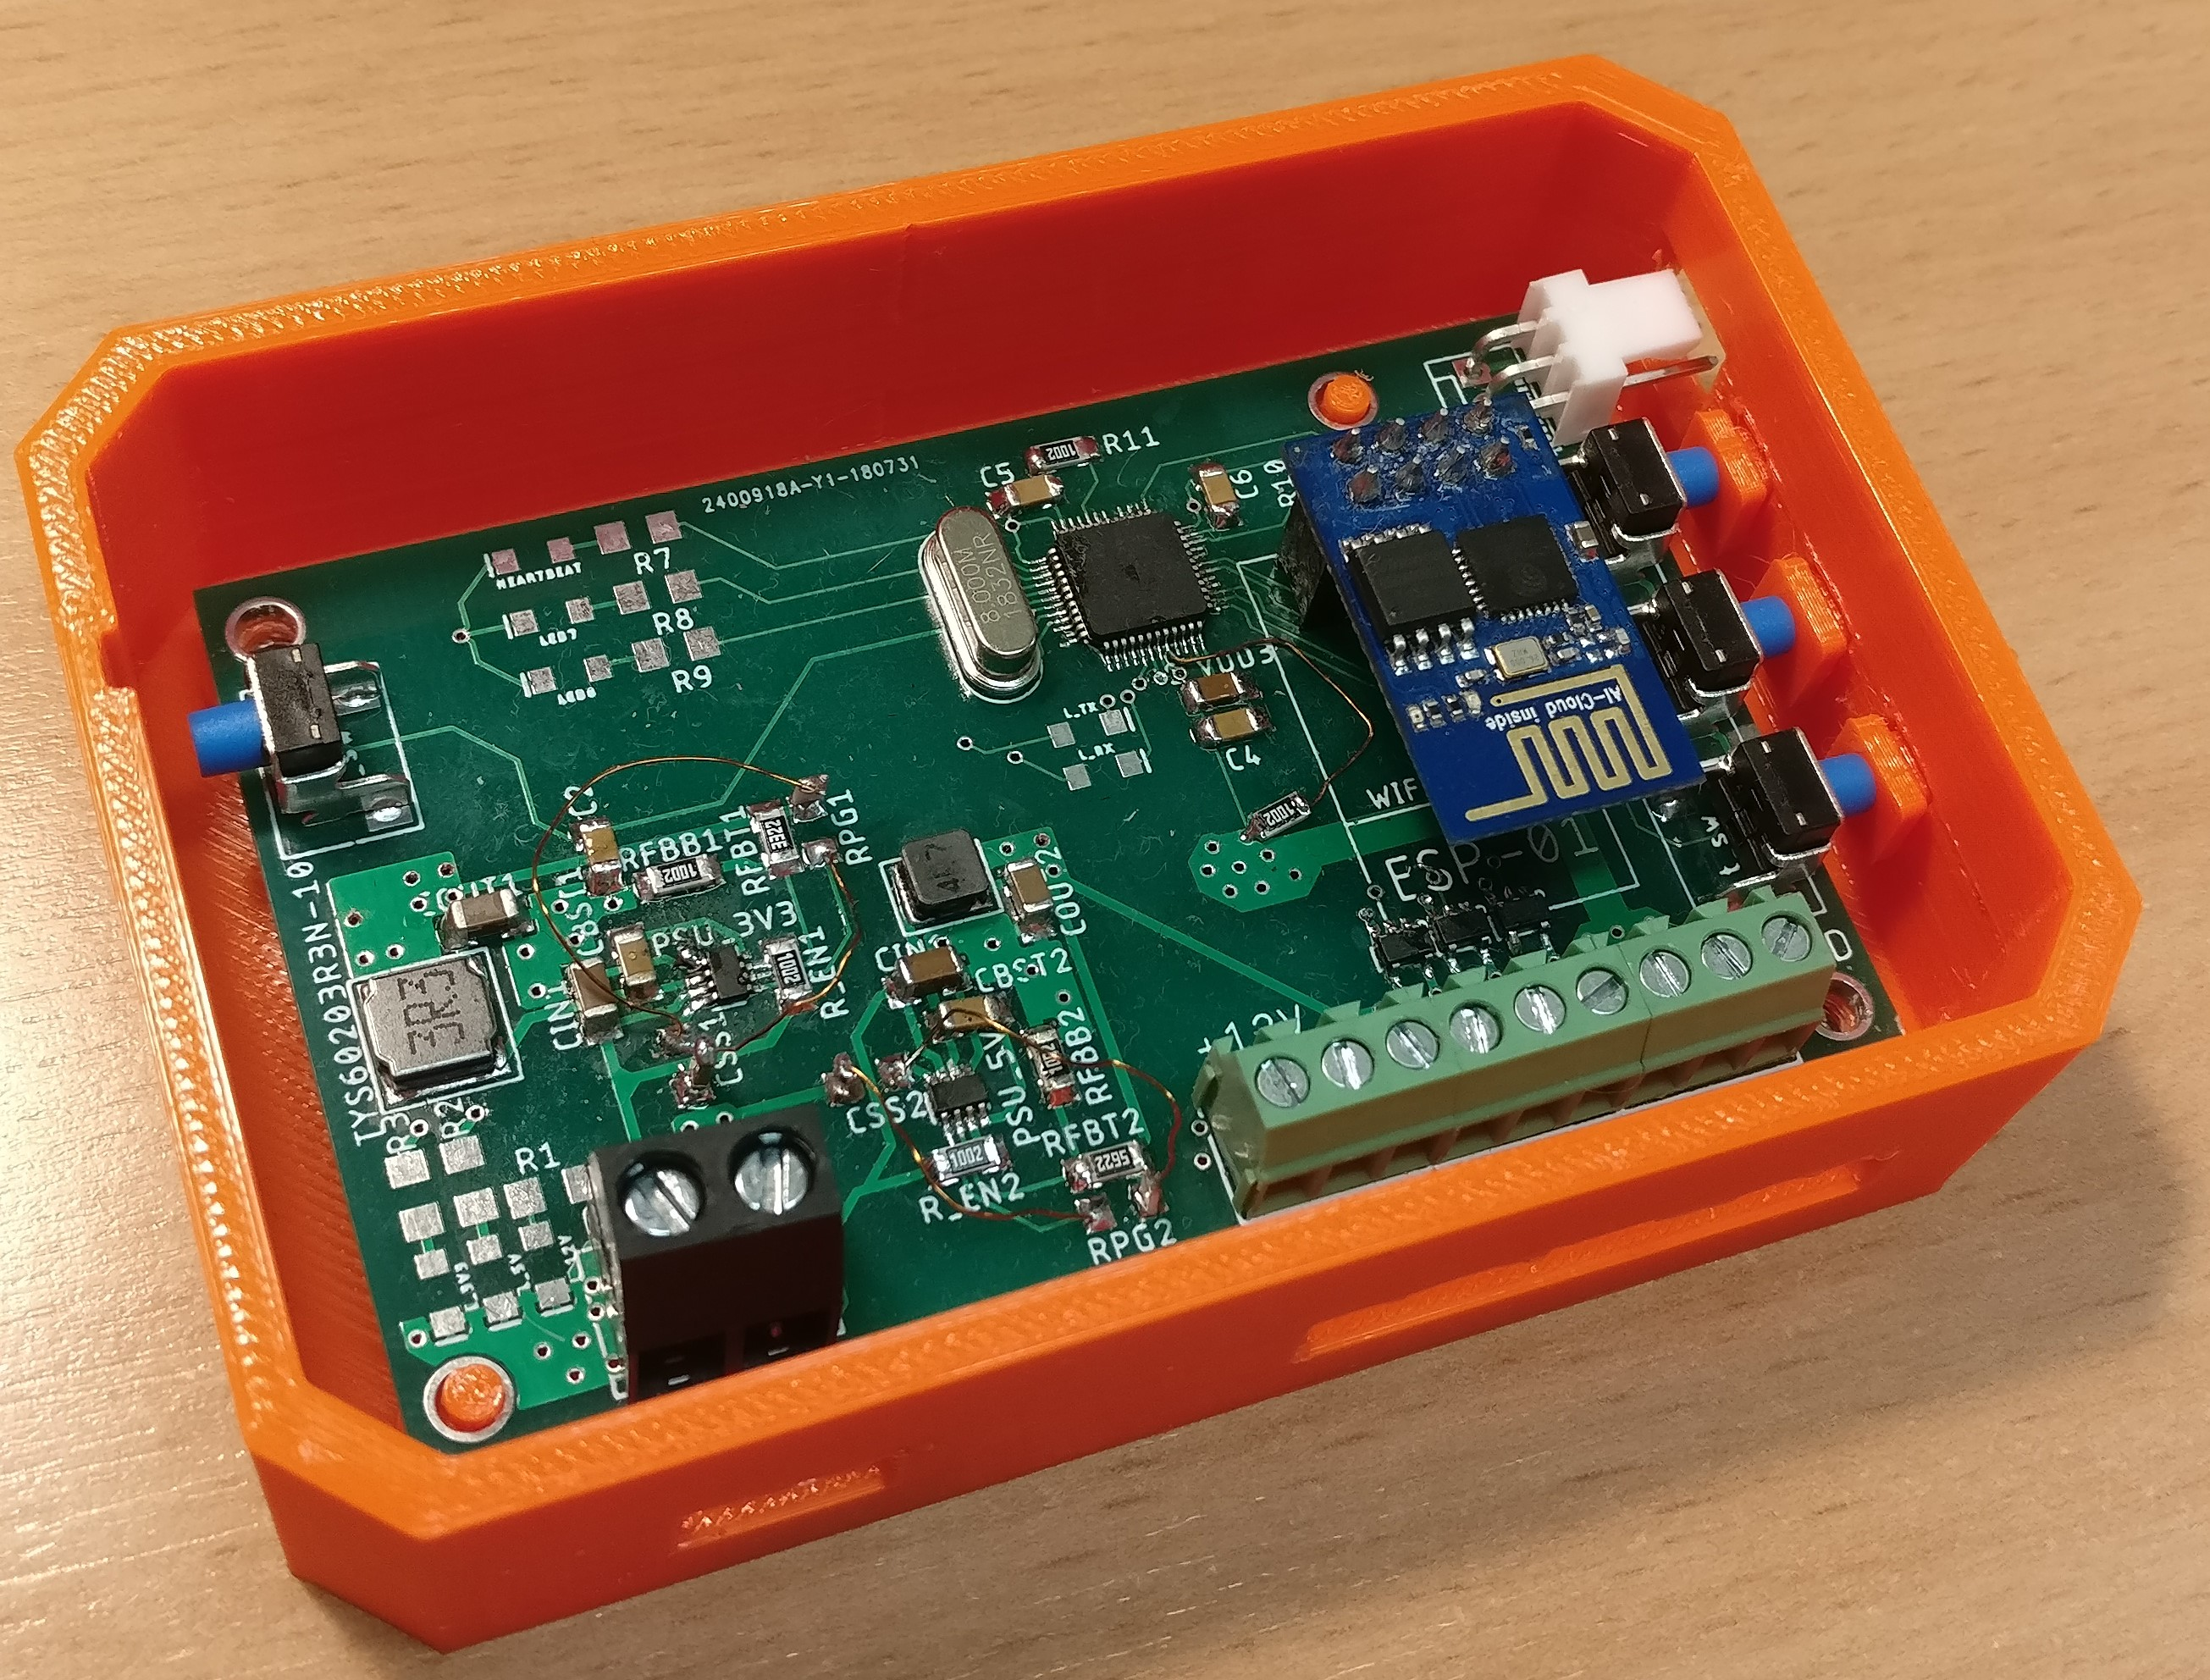
\includegraphics[height=5.5cm]{resources/pcb_res/printed_case_ngen}
                    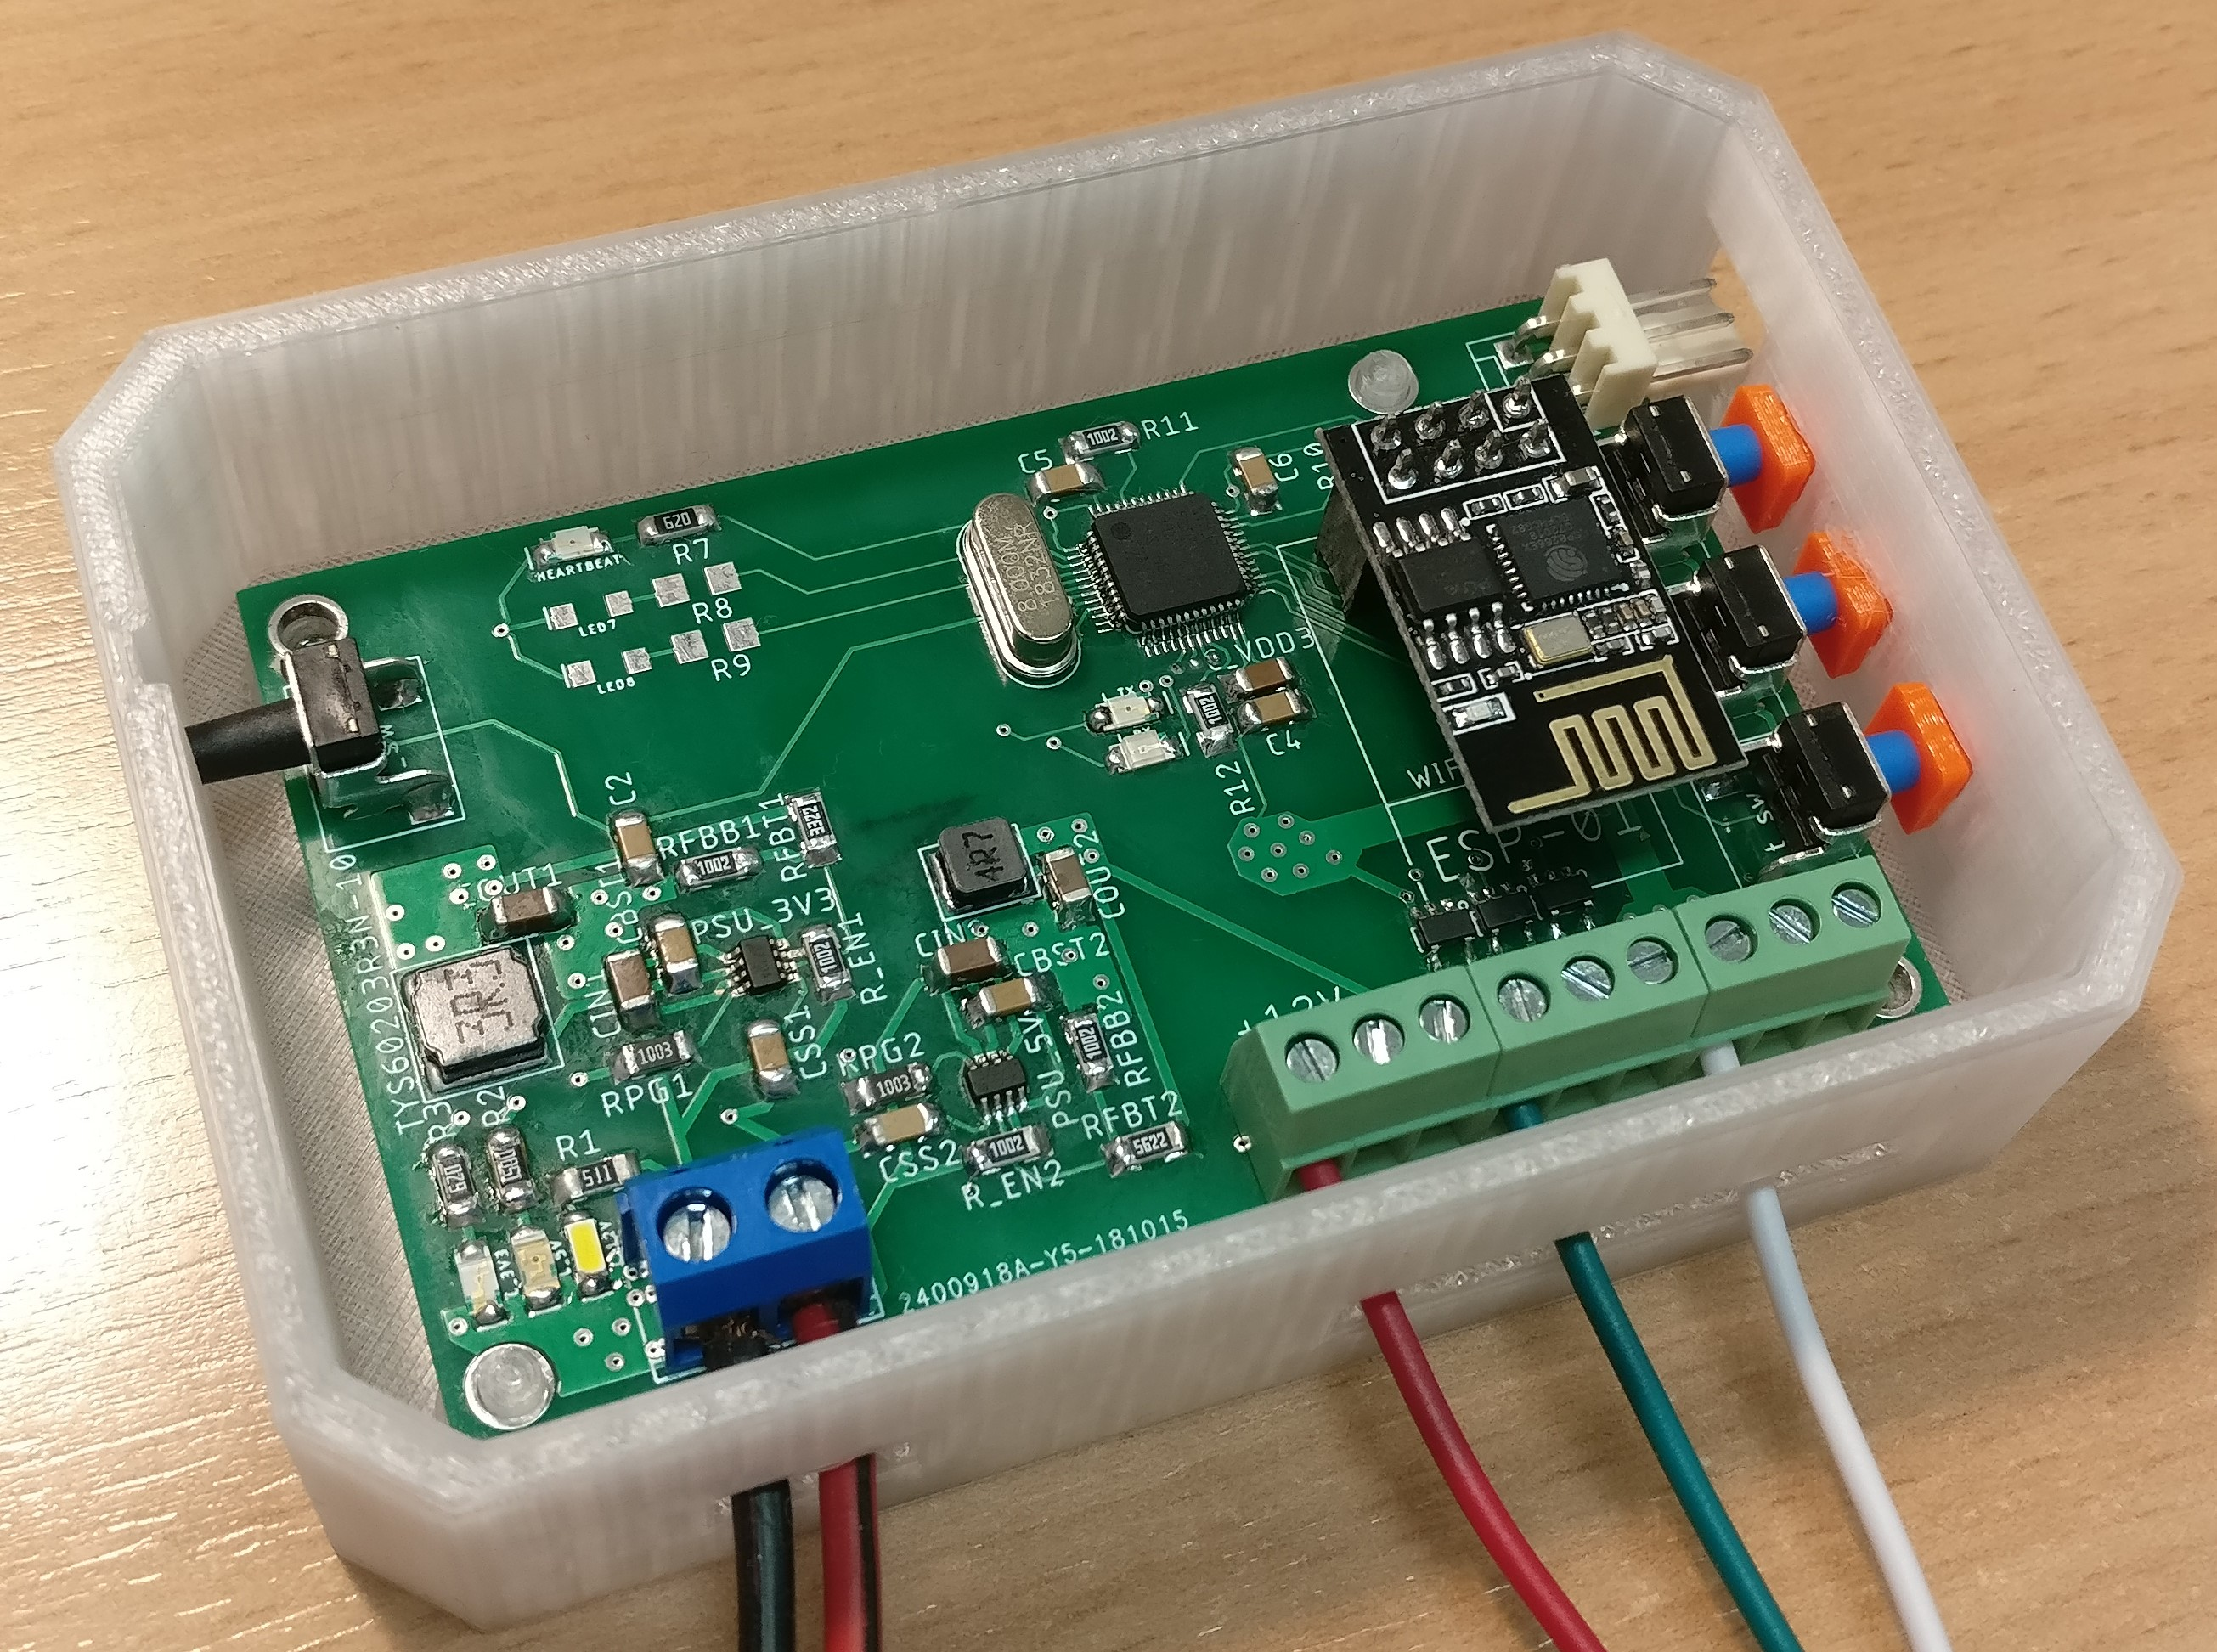
\includegraphics[height=5.5cm]{resources/pcb_res/printed_case_abs}
                    \caption{1. és 2. verziójú NYÁK-ok a 3D nyomtatott védő dobozukban}
                    \label{fig:printed_cases_1}
            \end{figure}
            
            \begin{figure}[h!]
                \centering
                    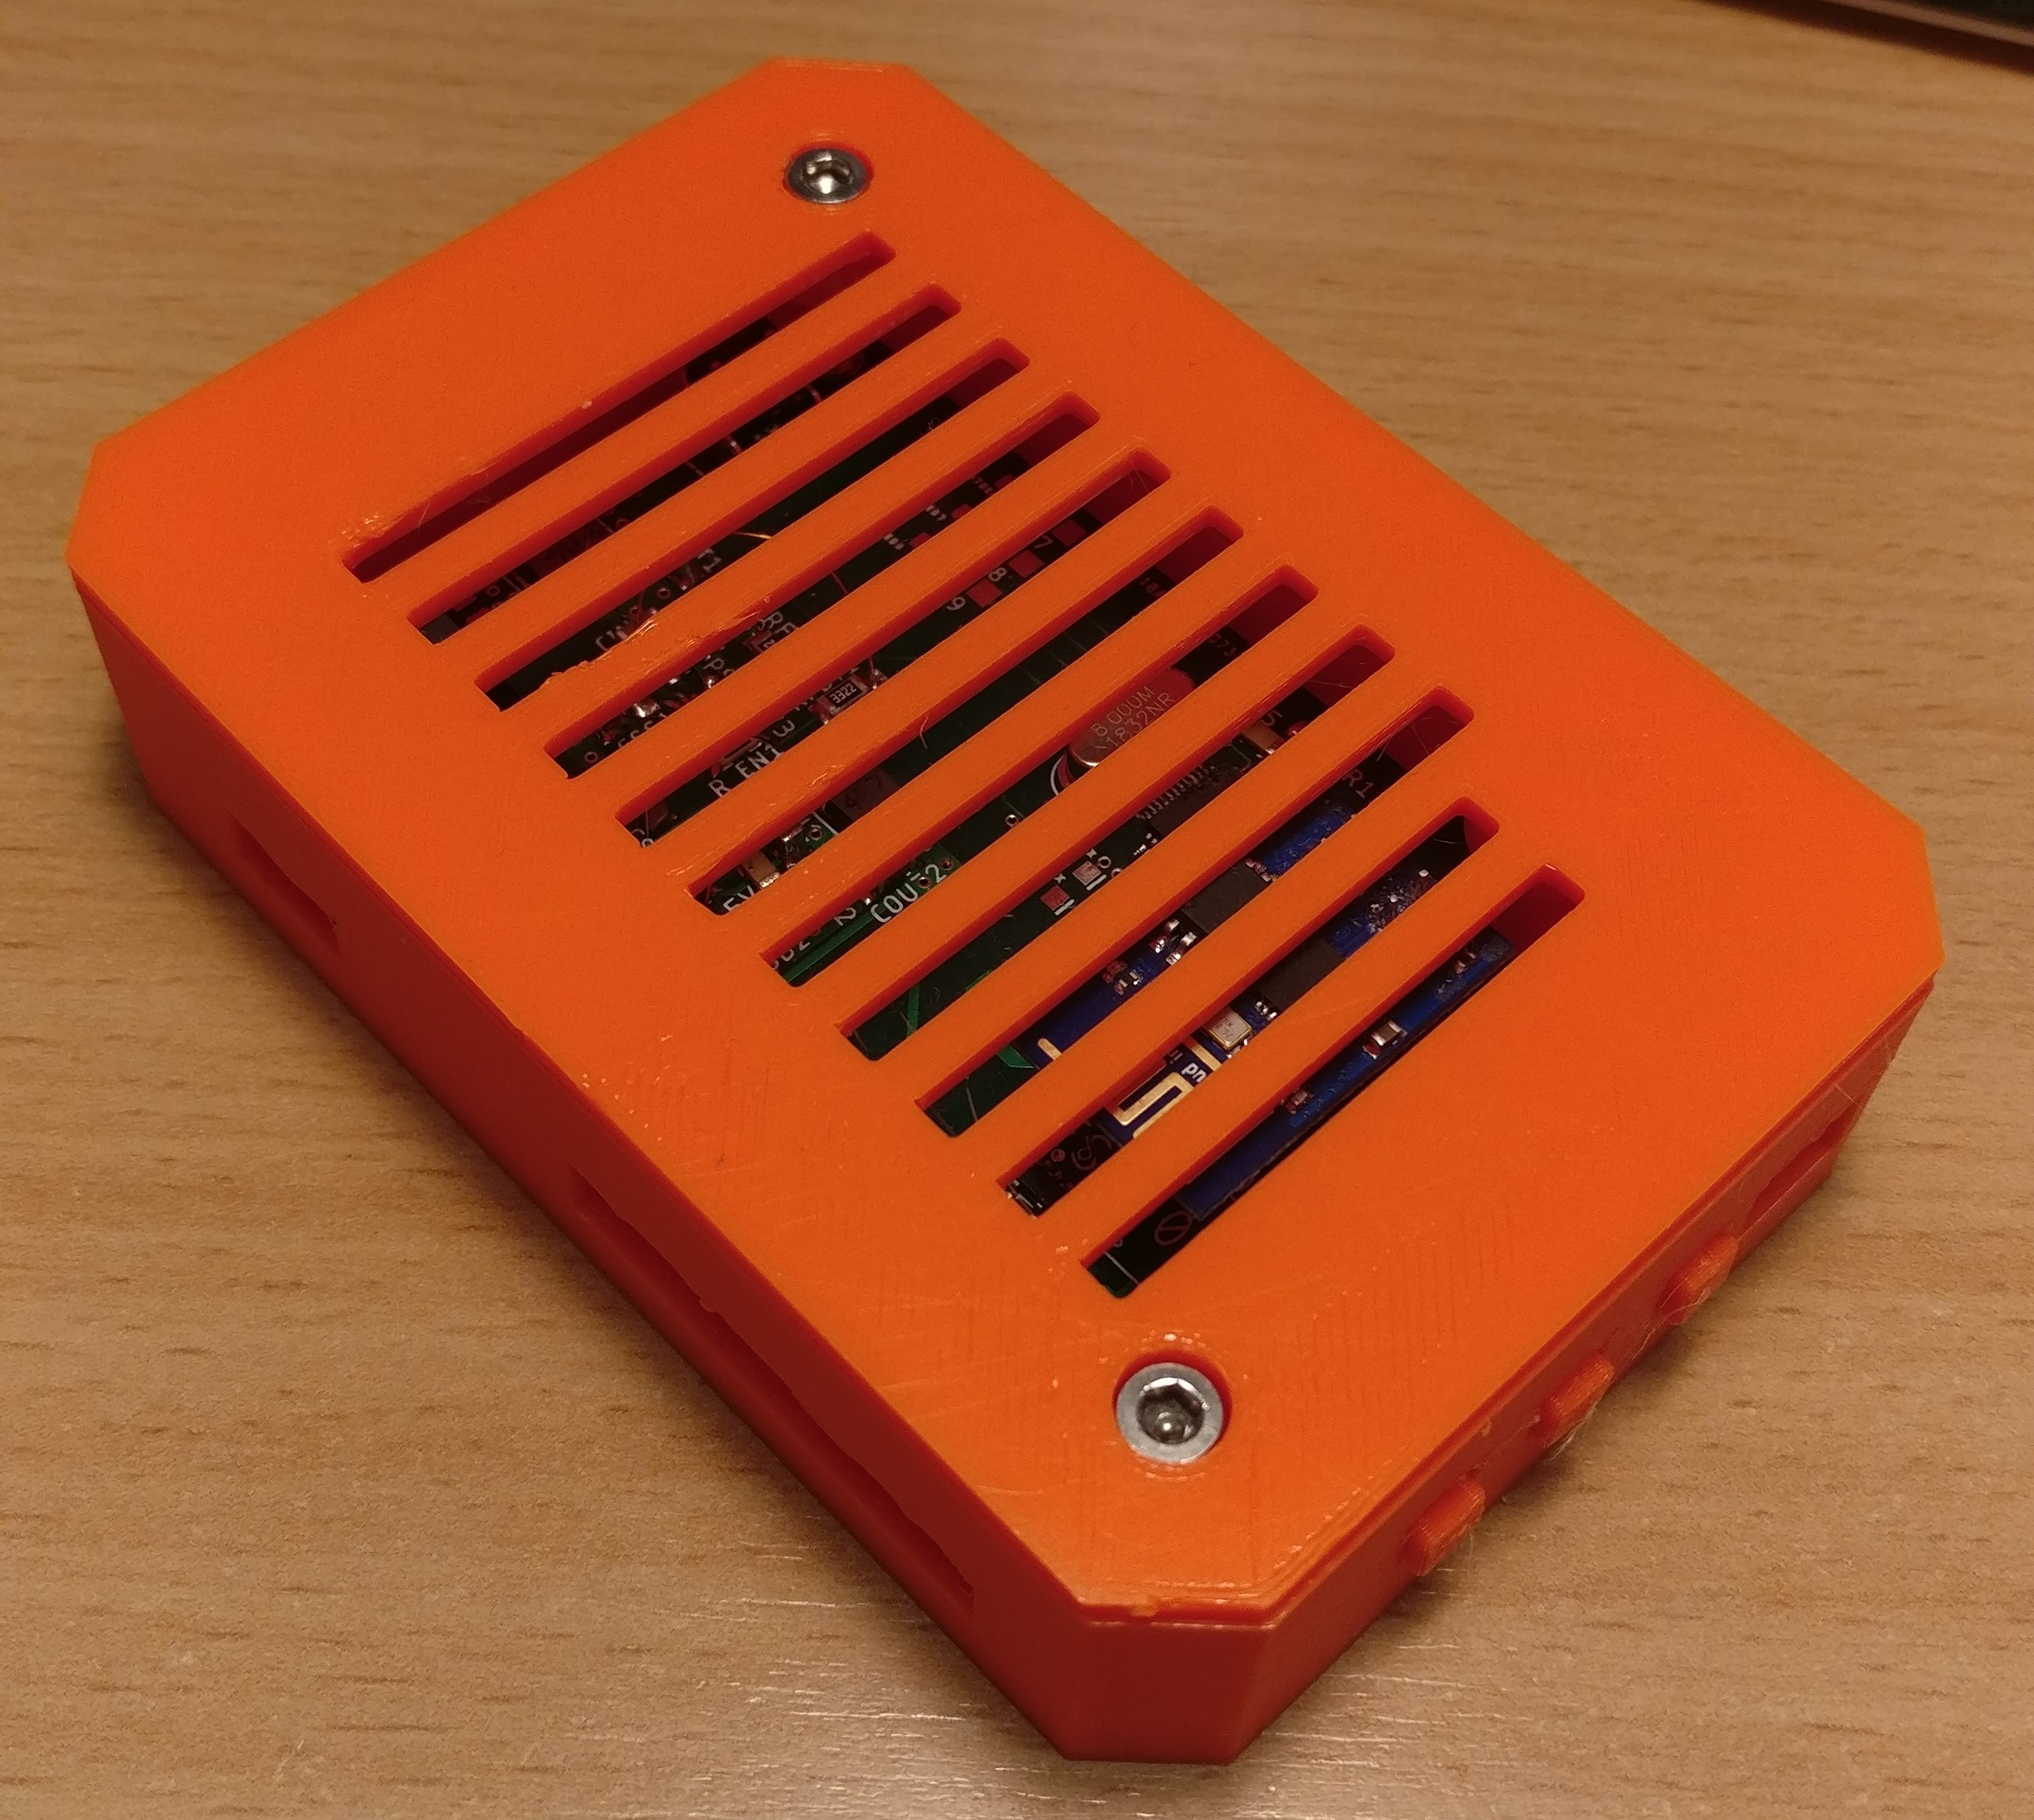
\includegraphics[height=6.5cm]{resources/pcb_res/printed_case_wtop_ngen}
                    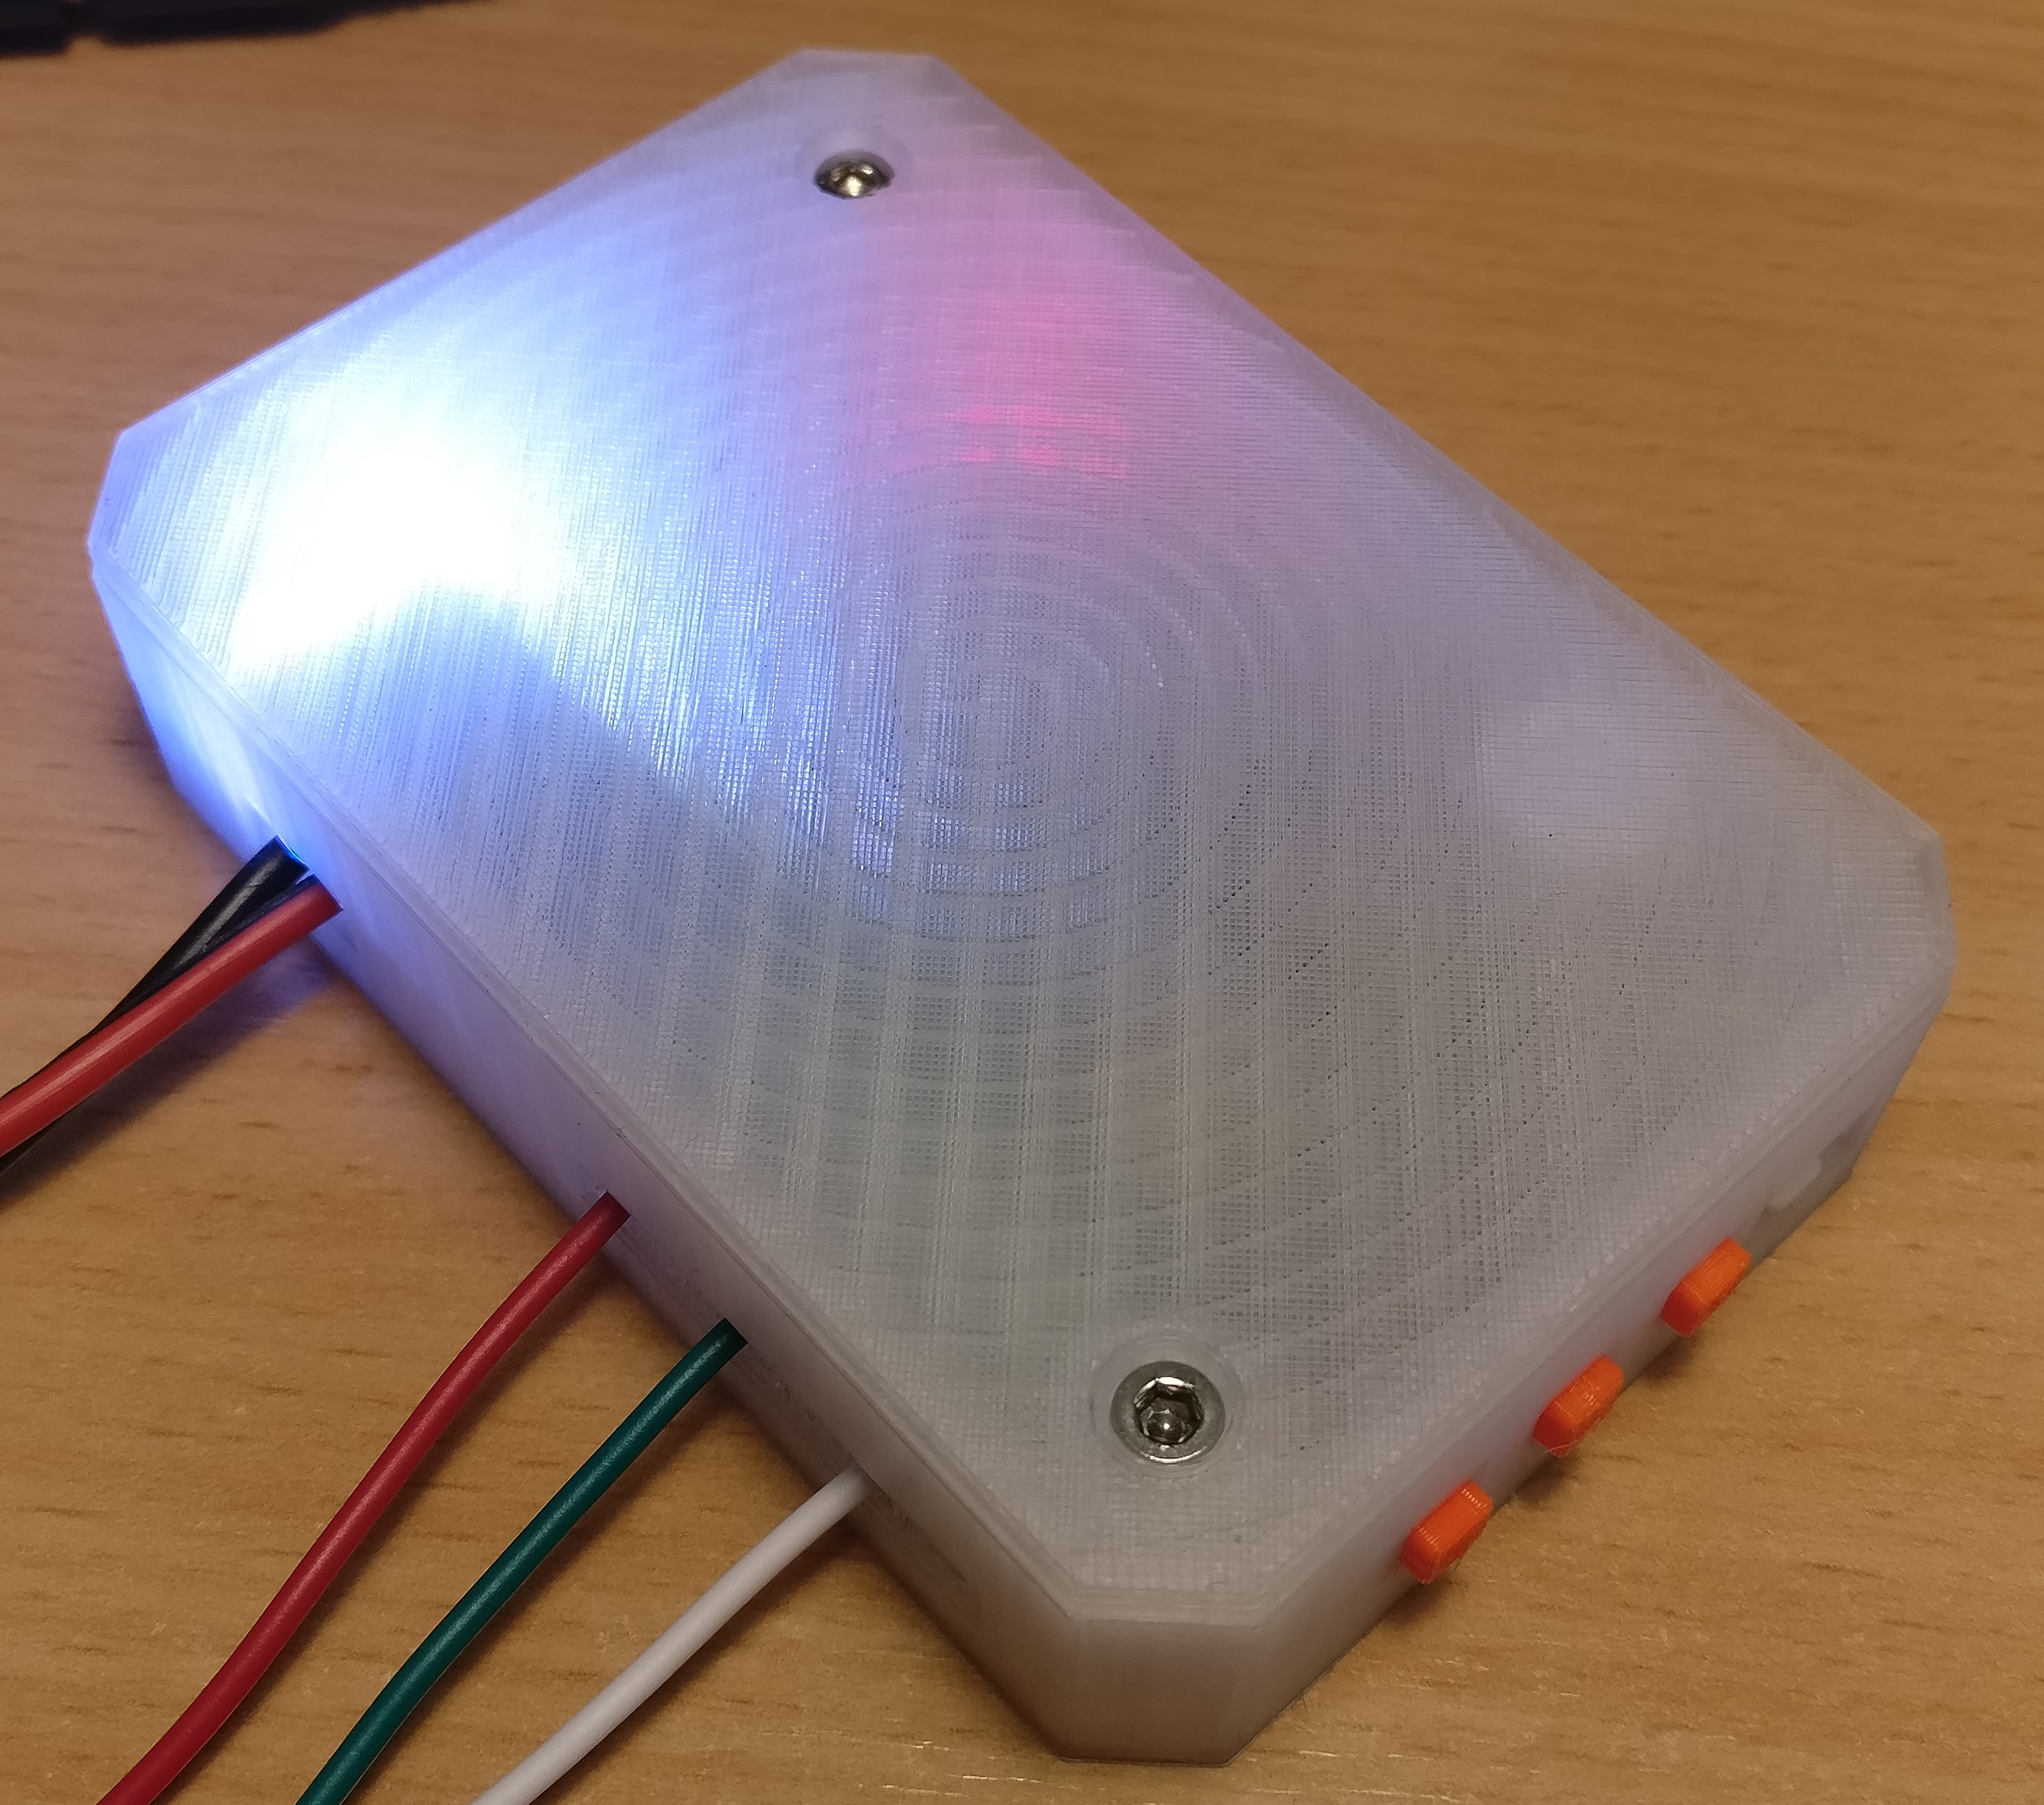
\includegraphics[height=6.5cm]{resources/pcb_res/printed_case_wtop_abs}
                    \caption{A 3D nyomtatott védő dobozok tetővel}
                    \label{fig:printed_cases_2}
            \end{figure}
    
otthoni megvalositas, aramforraskereses, bekotes, zavarszüres ferritgyuruvel, teraszrol kepek\\

\end{document}